%%%%%%%%%%%%%%%%%%%%%%%%%%%%%%%%%%%%%%%%
% datoteka diploma-FRI-vzorec.tex
%
%POZOR: ta verzija ne producira pdf datoteke v pdf/A formatu!!!
%namenjena je le za nalogo pri Diplomskem seminarju!
%
% vzorčna datoteka za pisanje diplomskega dela v formatu LaTeX
% na UL Fakulteti za računalništvo in informatiko
%
% na osnovi starejših verzij vkup spravil Franc Solina, maj 2021
% prvo verzijo je leta 2010 pripravil Gašper Fijavž
%
% za upravljanje z literaturo ta vezija uporablja BibLaTeX
%
% svetujemo uporabo Overleaf.com - na tej spletni implementaciji LaTeXa ta vzorec zagotovo pravilno deluje
%

\documentclass[a4paper,12pt,openright]{book}

\usepackage[a-1b]{pdfx}
\usepackage{url}
\usepackage{csquotes}
\hypersetup{pdftex, colorlinks=true, citecolor=black, filecolor=black, linkcolor=black, urlcolor=black, pdfproducer={LaTeX}, pdfcreator={LaTeX}}
 % konec pdf/A konfiguracije

\usepackage[utf8]{inputenc}   % omogoča uporabo slovenskih črk kodiranih v formatu UTF-8
\usepackage[english]{babel}    % naloži, med drugim, slovenske delilne vzorce
\usepackage[pdftex]{graphicx}  % omogoča vlaganje slik različnih formatov
\usepackage{fancyhdr}          % poskrbi, na primer, za glave strani
\usepackage{amssymb}           % dodatni matematični simboli
\usepackage{amsmath}           % eqref, npr.
\usepackage{csquotes}

\usepackage{color}
\usepackage{soul}
\usepackage{caption}
\captionsetup{font=small}
\let\oldtable\table
\let\endoldtable\endtable
\renewenvironment{table}[1][htbp] % redefine table environment
{
    \oldtable[#1]
    \footnotesize                     % sets all content in table smaller
}
{
    \endoldtable
}

\graphicspath{{../results_eng/}}

\usepackage{float}
\usepackage{booktabs}
\usepackage{xcolor}
\usepackage{makecell}
\definecolor{Apricot}{RGB}{251, 206, 177}

\iffalse
\usepackage[
backend=biber,
style=authoryear,
sorting=nty,
]{biblatex}
\fi

\usepackage[authoryear,round]{natbib}
\setcitestyle{aysep={},yysep={;}}

%\addbibresource{literatura.bib} %Imports bibliography file


%%%%%%%%%%%%%%%%%%%%%%%%%%%%%%%%%%%%%%%%
%	DIPLOMA INFO
%%%%%%%%%%%%%%%%%%%%%%%%%%%%%%%%%%%%%%%%
\newcommand{\ttitle}{Reinforcement learning on spiking neural networks}
\newcommand{\ttitleEn}{Reinforcement learning on spiking neural networks}
\newcommand{\tsubject}{\ttitle}
\newcommand{\tsubjectEn}{\ttitleEn}
\newcommand{\tauthor}{Matjaž Pogačnik}
\newcommand{\tkeywords}{spiking neural networks, reinforcement learning, R-STDP learning, TD learning}
\newcommand{\tkeywordsEn}{spiking neural networks, reinforcement learning, R-STDP learning, TD learning}

%%%%%%%%%%%%%%%%%%%%%%%%%%%%%%%%%%%%%%%%
%	HYPERREF SETUP
%%%%%%%%%%%%%%%%%%%%%%%%%%%%%%%%%%%%%%%%
\hypersetup{pdftitle={\ttitle}}
\hypersetup{pdfsubject=\ttitleEn}
\hypersetup{pdfauthor={\tauthor}}
\hypersetup{pdfkeywords=\tkeywordsEn}

%%%%%%%%%%%%%%%%%%%%%%%%%%%%%%%%%%%%%%%%
% postavitev strani
%%%%%%%%%%%%%%%%%%%%%%%%%%%%%%%%%%%%%%%%  

\addtolength{\marginparwidth}{-20pt} % robovi za tisk
\addtolength{\oddsidemargin}{40pt}
\addtolength{\evensidemargin}{-40pt}

\renewcommand{\baselinestretch}{1.3} % ustrezen razmik med vrsticami
\setlength{\headheight}{15pt}        % potreben prostor na vrhu
\renewcommand{\chaptermark}[1]%
{\markboth{\MakeUppercase{\thechapter.\ #1}}{}} \renewcommand{\sectionmark}[1]%
{\markright{\MakeUppercase{\thesection.\ #1}}} \renewcommand{\headrulewidth}{0.5pt} \renewcommand{\footrulewidth}{0pt}
\fancyhf{}
\fancyhead[LE,RO]{\sl \thepage} 
%\fancyhead[LO]{\sl \rightmark} \fancyhead[RE]{\sl \leftmark}
\fancyhead[RE]{\sc \tauthor}              % dodal Solina
\fancyhead[LO]{\sc Bachelor's thesis}     % dodal Solina


\newcommand{\BibLaTeX}{{\sc Bib}\LaTeX}
\newcommand{\BibTeX}{{\sc Bib}\TeX}

%%%%%%%%%%%%%%%%%%%%%%%%%%%%%%%%%%%%%%%%
% naslovi
%%%%%%%%%%%%%%%%%%%%%%%%%%%%%%%%%%%%%%%%  

\newcommand{\autfont}{\Large}
\newcommand{\titfont}{\LARGE\bf}
\newcommand{\clearemptydoublepage}{\newpage{\pagestyle{empty}\cleardoublepage}}
\setcounter{tocdepth}{1}	      % globina kazala

%%%%%%%%%%%%%%%%%%%%%%%%%%%%%%%%%%%%%%%%
% konstrukti
%%%%%%%%%%%%%%%%%%%%%%%%%%%%%%%%%%%%%%%%  
\newtheorem{izrek}{Theorem}[chapter]
\newtheorem{trditev}{Proposition}[izrek]
\newenvironment{dokaz}{\emph{Proof.}\ }{\hspace{\fill}{$\Box$}}


% %%%%%%%%%%%%%%%%%%%%%%%%%%%%%%%%%%%%%%%%%%%%%%%%%%%%%%%%%%%%%%%%%%%%%%%%%%%%%%%
% %% PDF-A
% %%%%%%%%%%%%%%%%%%%%%%%%%%%%%%%%%%%%%%%%%%%%%%%%%%%%%%%%%%%%%%%%%%%%%%%%%%%%%%%
%
% %%%%%%%%%%%%%%%%%%%%%%%%%%%%%%%%%%%%%%%%
% % define medatata
% %%%%%%%%%%%%%%%%%%%%%%%%%%%%%%%%%%%%%%%%
% \def\Title{\ttitle}
% \def\Author{\tauthor, matjaz.kralj@fri.uni-lj.si}
% \def\Subject{\ttitleEn}
% \def\Keywords{\tkeywordsEn}
%
% %%%%%%%%%%%%%%%%%%%%%%%%%%%%%%%%%%%%%%%%
% % \convertDate converts D:20080419103507+02'00' to 2008-04-19T10:35:07+02:00
% %%%%%%%%%%%%%%%%%%%%%%%%%%%%%%%%%%%%%%%%
% \def\convertDate{%
%     \getYear
% }
%
% {\catcode`\D=12
%  \gdef\getYear D:#1#2#3#4{\edef\xYear{#1#2#3#4}\getMonth}
% }
% \def\getMonth#1#2{\edef\xMonth{#1#2}\getDay}
% \def\getDay#1#2{\edef\xDay{#1#2}\getHour}
% \def\getHour#1#2{\edef\xHour{#1#2}\getMin}
% \def\getMin#1#2{\edef\xMin{#1#2}\getSec}
% \def\getSec#1#2{\edef\xSec{#1#2}\getTZh}
% \def\getTZh +#1#2{\edef\xTZh{#1#2}\getTZm}
% \def\getTZm '#1#2'{%
%     \edef\xTZm{#1#2}%
%     \edef\convDate{\xYear-\xMonth-\xDay T\xHour:\xMin:\xSec+\xTZh:\xTZm}%
% }
%
% %\expandafter\convertDate\pdfcreationdate
%
% %%%%%%%%%%%%%%%%%%%%%%%%%%%%%%%%%%%%%%%%
% % get pdftex version string
% %%%%%%%%%%%%%%%%%%%%%%%%%%%%%%%%%%%%%%%%
% \newcount\countA
% \countA=\pdftexversion
% \advance \countA by -100
% \def\pdftexVersionStr{pdfTeX-1.\the\countA.\pdftexrevision}
%
%
% %%%%%%%%%%%%%%%%%%%%%%%%%%%%%%%%%%%%%%%%
% % XMP data
% %%%%%%%%%%%%%%%%%%%%%%%%%%%%%%%%%%%%%%%%
% \usepackage{xmpincl}
% %\includexmp{pdfa-1b}
%
% %%%%%%%%%%%%%%%%%%%%%%%%%%%%%%%%%%%%%%%%
% % pdfInfo
% %%%%%%%%%%%%%%%%%%%%%%%%%%%%%%%%%%%%%%%%
% \pdfinfo{%
%     /Title    (\ttitle)
%     /Author   (\tauthor, damjan@cvetan.si)
%     /Subject  (\ttitleEn)
%     /Keywords (\tkeywordsEn)
%     /ModDate  (\pdfcreationdate)
%     /Trapped  /False
% }

%%%%%%%%%%%%%%%%%%%%%%%%%%%%%%%%%%%%%%%%
% znaki za copyright stran
%%%%%%%%%%%%%%%%%%%%%%%%%%%%%%%%%%%%%%%%  

\newcommand{\CcImageCc}[1]{%
	
\includegraphics[scale=#1]{cc_cc_30.pdf}%
}
\newcommand{\CcImageBy}[1]{%
	
\includegraphics[scale=#1]{cc_by_30.pdf}%
}
\newcommand{\CcImageSa}[1]{%
	
\includegraphics[scale=#1]{cc_sa_30.pdf}%
}

%%%%%%%%%%%%%%%%%%%%%%%%%%%%%%%%%%%%%%%%%%%%%%%%%%%%%%%%%%%%%%%%%%%%%%%%%%%%%%%
%%%%%%%%%%%%%%%%%%%%%%%%%%%%%%%%%%%%%%%%%%%%%%%%%%%%%%%%%%%%%%%%%%%%%%%%%%%%%%%

\begin{document}
\selectlanguage{english}
\frontmatter
\setcounter{page}{1} %
\renewcommand{\thepage}{}       % preprečimo težave s številkami strani v kazalu

%%%%%%%%%%%%%%%%%%%%%%%%%%%%%%%%%%%%%%%%
%naslovnica
 \thispagestyle{empty}%
   \begin{center}
    {\large\sc University of Ljubljana\\%
%      Fakulteta za elektrotehniko\\% za študijski program Multimedija
%      Fakulteta za upravo\\% za študijski program Upravna informatika
      Faculty of Computer and Information Science\\%
%      Fakulteta za matematiko in fiziko\\% za študijski program Računalništvo in matematika
     }
    \vskip 10em%
    {\autfont \tauthor\par}%
    {\titfont \ttitle \par}%
    {\vskip 3em \textsc{BACHELOR'S THESIS\\[5mm]         % dodal Solina za ostale študijske programe
%    VISOKOŠOLSKI STROKOVNI ŠTUDIJSKI PROGRAM\\ PRVE STOPNJE\\ RAČUNALNIŠTVO IN INFORMATIKA}\par}%
     UNIVERSITY STUDY PROGRAM\\ FIRST CYCLE\\ COMPUTER AND INFORMATION SCIENCE}\par}%
%    INTERDISCIPLINARNI UNIVERZITETNI\\ ŠTUDIJSKI PROGRAM PRVE STOPNJE\\ MULTIMEDIJA}\par}%
%    INTERDISCIPLINARNI UNIVERZITETNI\\ ŠTUDIJSKI PROGRAM PRVE STOPNJE\\ UPRAVNA INFORMATIKA}\par}%
%    INTERDISCIPLINARNI UNIVERZITETNI\\ ŠTUDIJSKI PROGRAM PRVE STOPNJE\\ RAČUNALNIŠTVO IN MATEMATIKA}\par}%
    \vfill\null%
% izberite pravi habilitacijski naziv mentorja!
    {\large \textsc{Supervisor}: prof. dr. Zoran Bosnić\par}%
%   {\large \textsc{Somentor}:  viš. pred./doc./izr. prof./prof. dr.  Martin Krpan \par}%
    {\vskip 2em \large Ljubljana, \the\year \par}%
\end{center}
% prazna stran
%\clearemptydoublepage      
% izjava o licencah itd. se izpiše na hrbtni strani naslovnice

%%%%%%%%%%%%%%%%%%%%%%%%%%%%%%%%%%%%%%%%
%copyright stran
%%%%%%%%%%%%%%%%%%%%%%%%%%%%%%%%%%%%%%%%
\newpage
\thispagestyle{empty}

\vspace*{5cm}
{\small \noindent
This work is offered under the license \textit{Creative Commons Attribution-ShareAlike 2.5 Slovenia} (or any later version).
This means that the text, images, graphs, and other components of the work, as well as the results of the bachelor's thesis, may be freely distributed,
reproduced, used, communicated to the public, and adapted, provided that the author and title of this
work are clearly and visibly stated and that, in the event of modification, transformation, or use of this work in another work, the adaptation may be distributed only under
the same license.
License details are available at \href{http://creativecommons.si}{creativecommons.si} or at the Institute for
Intellectual Property, Streli\v ska 1, 1000 Ljubljana.

\vspace*{1cm}
\begin{center}% 0.66 / 0.89 = 0.741573033707865
\CcImageCc{0.741573033707865}\hspace*{1ex}\CcImageBy{1}\hspace*{1ex}\CcImageSa{1}%
\end{center}
}

\vspace*{1cm}
{\small \noindent
The source code of the bachelor's thesis, its results, and the software developed for this purpose are offered under the GNU General Public License,
version 3 (or any later version). This means that it may be freely distributed and/or modified under its terms.
License details are available at \url{http://www.gnu.org/licenses/}.
}

\vfill
\begin{center} 
\ \\ \vfill
{\em
The text was typeset using the \LaTeX\ text editor.}
\end{center}

% prazna stran
\clearemptydoublepage

%%%%%%%%%%%%%%%%%%%%%%%%%%%%%%%%%%%%%%%%
% stran 3 med uvodnimi listi
\thispagestyle{empty}
\
\vfill

\bigskip
\noindent\textbf{Candidate:} Matjaž Pogačnik\\
\noindent\textbf{Title:} Reinforcement learning on spiking neural networks\\
% vstavite ustrezen naziv študijskega programa!
\noindent\textbf{Type of thesis:} Bachelor's thesis in the first-cycle university program Computer and Information Science \\
% izberite pravi habilitacijski naziv mentorja!
\noindent\textbf{Supervisor:} prof. dr. Zoran Bosnić\\
% \noindent\textbf{Somentor:} isto kot za mentorja

\bigskip
\noindent\textbf{Description:}\\
The candidate should study the principles of spiking neural networks and reinforcement learning approaches suitable for such models. They should develop and implement a selected learning algorithm and evaluate it experimentally in a chosen problem environment. The results should be analyzed and compared with existing approaches.

\vfill



\vspace{2cm}

% prazna stran
\clearemptydoublepage

% TODO: zahvala
% zahvala
\iffalse
\thispagestyle{empty}\mbox{}\vfill\null\it%
\noindent
At this place, write whom you thank for help with preparing the bachelor's thesis or with your studies in general. Be careful not to forget anyone. They might hold it against you. This can be avoided by omitting the entire acknowledgment.
\rm\normalfont

% prazna stran
\clearemptydoublepage
\fi

%%%%%%%%%%%%%%%%%%%%%%%%%%%%%%%%%%%%%%%%
% posvetilo, če sama zahvala ne zadošča :-)
%\thispagestyle{empty}\mbox{}{\vskip0.20\textheight}\mbox{}\hfill\begin{minipage}{0.55\textwidth}%
%Svoji dragi Alenčici.
%\normalfont\end{minipage}

% prazna stran
%\clearemptydoublepage


%%%%%%%%%%%%%%%%%%%%%%%%%%%%%%%%%%%%%%%%
% kazalo
\pagestyle{empty}
\def\thepage{}% preprečimo težave s številkami strani v kazalu
\tableofcontents{}


% prazna stran
\clearemptydoublepage

%%%%%%%%%%%%%%%%%%%%%%%%%%%%%%%%%%%%%%%%
% seznam kratic

\chapter*{List of abbreviations}

\noindent\begin{tabular}{p{0.30\textwidth}|p{.70\textwidth}}    % po potrebi razširi prvo kolono tabele na račun drugih dveh!
  {\bf abbreviation} & {\bf English} \\ \hline
  {\bf IAF} & Integrate and fire \\
  {\bf LIF} & Leaky integrate and fire \\
  {\bf STDP} & Spike timing dependent plasticity \\
  {\bf R-STDP} & Reward modulated spike timing dependent plasticity \\
  {\bf TD}   & Temporal difference \\
%  \dots & \dots & \dots \\
\end{tabular}


% prazna stran
\clearemptydoublepage

%%%%%%%%%%%%%%%%%%%%%%%%%%%%%%%%%%%%%%%%
% abstract
\selectlanguage{english}
\addcontentsline{toc}{chapter}{Abstract}
\chapter*{Abstract}

\noindent\textbf{Title:} \ttitleEn
\bigskip

\noindent\textbf{Author:} \tauthor
\bigskip

%\noindent\textbf{Abstract:} 
\noindent %This sample document presents an approach to typesetting your BSc thesis using \LaTeX. 
%A proper abstract should contain around 100 words which makes this one way too short.
In this thesis, we study reinforcement learning in spiking neural networks, a type of neural network that behaves similarly to the human brain. We present and address key challenges in training spiking networks and develop solutions that account for both biological plausibility and simulation complexity. By adapting the classical form of reward modulated spike timing dependent plasticity (\textit{R-STDP}), we enable efficient learning and the assignment of credit to past decisions, while preserving the core principle of R-STDP, in which synapses encode the influence of past neuronal activity on selected actions, without introducing negative rewards or unrealistic mechanisms.

We then extend the developed system into an actor-critic architecture, enabling it to solve problems with delayed rewards by propagating the expected reward from the goal back to previous states. The system is first evaluated on simplified tasks and then on more complex problems, such as the game Pong and the gridworld problem. In Pong, the results show progressively longer sequences of play without missing the ball, while in the gridworld task the strategy gradually improves and the path to the goal becomes shorter.
\bigskip

\noindent\textbf{Keywords:} \tkeywordsEn.
\selectlanguage{english}
% prazna stran
\clearemptydoublepage

%%%%%%%%%%%%%%%%%%%%%%%%%%%%%%%%%%%%%%%%
\mainmatter
\setcounter{page}{1}
\pagestyle{fancy}

\chapter{Introduction}
\label{intro}
Spiking neural networks represent a class of neural networks whose operation is based on discrete spikes and pronounced temporal dynamics. Unlike classical artificial neural networks, which process information with continuous activations in discrete layers, spiking neural networks are based on asynchronous events in time, which makes them closer to the actual functioning of biological brains. Their key advantage is not only potential computational efficiency, but above all the possibility of modeling known biological mechanisms, such as temporal signal integration, synaptic plasticity, and neuromodulation.

Research on spiking neural networks is meaningful both from the perspective of artificial intelligence and computational neuroscience. Such models make it possible to study how meaningful behavior can emerge from local learning rules based on the activity of individual neurons and synapses, together with global reward signals. In this way, artificial intelligence moves closer to understanding learning in the behavioral sense, where the system does not optimize a predefined function but gradually adapts and forms operating strategies through interaction with the environment.

An especially important framework for such learning is reinforcement learning, which in biological systems is closely linked to the functioning of the dopamine system. While reinforcement learning algorithms are well established in classical machine learning, their direct use in spiking neural networks is not possible because of the different nature of signals, pronounced temporal dependence, and requirements for biological plausibility. This raises the question of how to design learning mechanisms that are both effective for solving tasks and consistent with known processes in the brain.

The central problem addressed in this work is learning in spiking neural networks in environments with immediate and delayed rewards. Simpler mechanisms, such as \textit{reward modulated spike timing dependent plasticity} (\textit{R-STDP}), enable learning in cases where the reward follows the action directly, but fail on tasks where the reward is temporally distant. This gives rise to the problem of \textit{temporal credit assignment}, which represents one of the key challenges of reinforcement learning in biologically realistic models.

In this bachelor's thesis, we approach this problem gradually. First, in Chapter \ref{neuron_synapse_modelling}, we present and evaluate different neuron and synapse models that serve as a foundation for the further development of learning mechanisms. On this basis, in Section \ref{sec:rstdp}, we develop a reinforcement learning system based exclusively on spiking neural networks. By adapting the classical R-STDP synapse, we enable more effective credit assignment to past decisions, while preserving the basic principle of local learning. An important feature of the approach is the use of exclusively non-negative reward signals, since negative dopamine does not exist in biological dopamine systems; a decrease in dopamine activity represents the absence or reduction of expected reward, not a separate negative signal. This distinguishes our approach from many existing methods that use explicit negative rewards.

Because the described approach still does not enable effective solving of tasks with longer temporal reward dependencies, in Section \ref{sec:td_learning} we extend the developed system with \textit{temporal-difference learning} into a spiking actor-critic neural architecture inspired by dopamine circuits of the basal ganglia. In such a system, the actor is responsible for action selection, while the critic estimates the expected future reward of individual states and generates a learning signal for synaptic adaptation. This extension enables propagation of expected reward from goal states back to previous states, and thus effective learning in environments with delayed rewards. We evaluate the operation of the extended system on the gridworld problem, where the system gradually learns better strategies and shorter paths to the goal.

For this purpose, in Chapter \ref{neuron_synapse_modelling} we first present and evaluate different neuron and synapse models and their properties. Then, in Section \ref{sec:rstdp}, we develop a system based on an adapted R-STDP synapse that enables more effective credit assignment to past decisions in tasks with immediate rewards, which we show on the task of playing \href{https://en.wikipedia.org/wiki/Pong}{Pong}. Because such an approach still does not allow learning in environments with longer temporal reward dependence, in Section \ref{sec:td_learning} we extend the system with temporal-difference learning (\textit{TD} learning) into a spiking actor-critic neural architecture inspired by dopamine circuits of the basal ganglia. The extended system enables propagation of expected reward to previous states and is evaluated on the gridworld problem, where the agent gradually learns a more efficient strategy and shorter path to the goal.

\chapter{Field Overview and Related Work}
Research on spiking neural networks has developed in recent decades primarily at the intersection of artificial intelligence, neuroscience, and neuromorphic engineering. The central challenge in this field is learning, since classical gradient approaches used in artificial neural networks are not directly applicable due to the discrete nature of spikes and nonlinear temporal dynamics.

One of the fundamental approaches to learning in spiking neural networks is synaptic plasticity dependent on the time difference between spikes of pre- and postsynaptic neurons (\textit{spike timing dependent plasticity}, \textit{STDP}). Extensions of this mechanism with a global reward signal, such as R-STDP, enable the use of spiking neural networks in reinforcement learning. Such approaches are successful in tasks with immediate rewards, but they face limitations when solving problems with delayed rewards, where temporal propagation of the learning signal is required.

In the field of reinforcement learning, there is extensive literature addressing various tasks such as navigation, game playing, and robot control. \citet{robot} discuss the use of reinforcement learning in robotic systems, where an agent learns strategies based on interaction with a real, noisy environment. Similar approaches are also used in simulated environments, where properties of learning algorithms are studied, for example in the cart-pole problem \citet{vozicekSPalico} or in game playing \citet{predvidevanjeAkcij}. These works mostly use classical neural network models or symbolic state representations, while temporal dynamics are not explicitly modeled at the level of individual events.

Spiking neural networks differ from recurrent architectures such as LSTM or GRU in that time is not implicitly encoded in the network state, but is directly present in the form of temporal delays between spikes. This enables natural processing of event-driven and asynchronous signals, while also opening the possibility of energy-efficient implementation on neuromorphic hardware. Computation is therefore not based on sequential matrix multiplication, but on sparse events where only part of the network is updated when a spike occurs.

A particularly interesting research direction is linking spiking neural networks with temporal-difference learning. In \citet{pilotStudy}, the use of TD learning on a hard-wired (neuromorphic) spiking neural network is presented, where the final task is playing Pong. A hard-wired implementation means that the network is realized on specialized hardware, where neurons and synapses are physically implemented, which enables high energy efficiency while limiting model flexibility.

A biologically more direct implementation of TD learning is the actor-critic architecture, inspired by the functioning of the basal ganglia and dopamine system in the brain \citet{actorCritic}. In this framework, the critic estimates state values and generates a dopamine signal representing reward prediction error, while the actor adjusts the action-selection strategy on this basis. Such a reward system is closely linked to experimental findings on dopamine neuron function, where they encode the difference between expected and actual reward.

Compared with existing works, this bachelor's thesis focuses on a unified spiking neural architecture that combines local learning rules, global reward signals, and a biologically meaningful implementation without explicit negative rewards. The emphasis is on temporal credit assignment and the gradual extension of the basic R-STDP approach into an actor-critic architecture that enables learning in environments with delayed rewards.

\chapter{Modeling Neurons and Synapses}
\label{neuron_synapse_modelling}
Spiking neural networks are defined by a neuron model and a synapse model that connects neurons. There are many models; in what follows, two neuron models will be presented and compared with respect to their usefulness for reinforcement learning in spiking neural networks. A synapse model suitable for reinforcement learning will also be presented and used in the systems developed below.

Neuron models describe electrical properties of the neuron's cell membrane in the brain. Through synapses, neurons receive output (postsynaptic) currents from neurons to which they are connected and update their membrane potential over time according to synaptic weight. Current that arrives through a positively weighted synapse from the neuron at the beginning of the synapse (the presynaptic neuron) to the neuron at the end (the postsynaptic neuron) causes an increase in membrane potential. When a neuron's membrane potential exceeds $V_{th}$, a spike is fired, and this neuron releases its postsynaptic current into the synapse. This system is shown in Figure \ref{pre-sin-post}, where postsynaptic currents of presynaptic neurons $i_{\text{syn}}(t - t_j - d_j)$ are presented. Index $j$ denotes individual presynaptic neurons, $t$ represents the current time, $t_j$ the firing time of the presynaptic neuron's action potential, and $d_j$ the signal delay due to transmission through the synapse to the postsynaptic neuron.

\begin{figure}[htbp]
\begin{center}
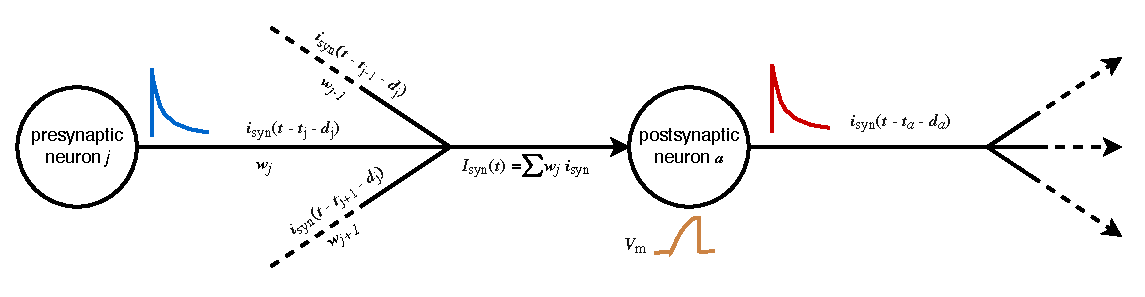
\includegraphics[width=1.0\textwidth]{neuron_models/pre-syn-post.pdf}
\end{center}
\caption{Illustration of pre- and postsynaptic relations and individual postsynaptic currents.}
\label{pre-sin-post}
\end{figure}

\noindent The membrane potential value decreases over time regardless of input currents due to leakage conductance $g_L$. Such neuron models are called current-driven leaky integrate-and-fire neuron models (\textit{leaky IAF}). After spike firing, the magnitude of the postsynaptic current changes according to a curve determined by the selected model kernel that represents the current shape after a spike. In the following, we present two approaches: a simpler model with an exponentially shaped postsynaptic current and a more complex model with alpha-shaped postsynaptic currents. Both are shown at equal parameters in Figure \ref{neuron_psc} and described in more detail below, together with parameters. Also marked is $36.8\%$ of the maximum value, which, according to calculations in Section \ref{eksponentno_jedro}, is reached by the exponential kernel exactly at the time when the alpha kernel reaches its maximum value.
\newpage
\begin{figure}[htbp]
\begin{center}

\includegraphics[width=1.0\textwidth]{neuron_models/PSCs}
\end{center}
\caption{Postsynaptic current of the model with an exponential and alpha kernel at synaptic weight $w=50$ and $\tau_{\text{syn, ex}}=5~\mathrm{ms}$. The exponential kernel causes an immediate jump of postsynaptic
current at spike firing and exponential decay, while the alpha kernel models
a gradual rise of current to a maximum and then a slower decline, which better reflects the temporal dynamics
of biological synapses.}
\label{neuron_psc}
\end{figure}
\noindent The membrane potential of a leaky IAF neuron (\textit{LIF neuron}) changes according to the balance between capacitance and leakage through membrane conductance, input currents $I_{\text{syn}}$, and external noise $I_e$. The membrane model that determines how the membrane potential changes is defined by the following parameters.

\begin{itemize}
    \item \textbf{$E_L$ --- resting membrane potential} \\
    The electrical potential to which the membrane potential relaxes in the absence of input currents;

    \item \textbf{$C_m$ --- membrane capacitance} \\
    Membrane capacitance, which determines how quickly the membrane potential responds to input currents;

    \item \textbf{$\tau_m$ --- membrane time constant} \\
    The time during which the membrane passively integrates current; defined as the ratio between capacitance $C_m$ and leakage conductance $g_L$. The constant $\tau_m$ can also be defined as the product of capacitance and membrane resistance $\tau_m = C_m R_m = \frac{C_m}{g_L}$;

    \item \textbf{$t_{ref}$ --- refractory period} \\
    The time during which the neuron cannot fire again after firing an action potential;

    \item \textbf{$V_{th}$ --- firing threshold} \\
    The membrane potential at which the neuron fires an action potential;

    \item \textbf{$V_{\min}$ --- lower membrane potential bound} \\
    Absolute lower bound for membrane potential;

    \item \textbf{$I_e$ --- external constant current} \\
    Additional current that models constant external noise.
\end{itemize}
The membrane potential $V_m$ in the current-driven leaky integrate-and-fire neuron model is described, with respect to the previously listed parameters, by the differential equation
\begin{equation*}
    \frac{dV_m}{dt}=-\frac{V_m-E_L}{\tau_m}+\frac{I_{\text{syn}}+I_e}{C_m}.
\end{equation*}
The first term on the right side of the equation describes passive leakage of the membrane potential toward the resting value $E_L$ with time constant $\tau_m$, which determines membrane relaxation speed. The second term represents the influence of input currents, where $I_{\text{syn}}$ denotes the total synaptic current generated by all presynaptic neurons, and $I_e$ denotes external constant current or noise. Membrane capacitance $C_m$ determines how strongly individual currents affect the change in membrane potential. The total current $I_{\text{syn}}$ that the postsynaptic neuron receives through all synapses can be split into two components according to synaptic weight values. If synaptic weight is positive, membrane potential will increase toward firing threshold according to postsynaptic current. Such a connection is called excitatory. Conversely, if synaptic weight is negative, membrane potential decreases. Such a connection is called inhibitory. In what follows, notation $I_{\text{syn}}$ and $i_{\text{syn}}$ will be split into $i_{\text{syn, ex}}$ and $i_{\text{syn, in}}$, written jointly as $i_{\text{syn, X}}$, where $X \in \{\text{ex, in}\}$, and $I_{\text{syn}}$ will be written as the sum of $I_{\text{syn, ex}}$ and $I_{\text{syn, in}}$. This more general notation enables the use of different synaptic time constants, defined below, for excitatory and inhibitory connections. We thus write $I_{\text{syn}}$ as

\[
I_{\text{syn}}(t) = I_{\text{syn, ex}}(t) + I_{\text{syn, in}}(t) ,
\]

\noindent where

\[
I_{\text{syn, X}}(t) = \sum_j w_j \sum_k i_{\text{syn, X}}(t - t_j^k - d_j) ,
\]

\noindent where $j$ runs over excitatory ($X = \text{ex}$) and inhibitory ($X = \text{in}$) synapses with weights $w_j$ to presynaptic neurons, and $k$ runs over spike times of neuron $j$. $d_j$ represents delay due to signal travel through the synapse to neuron $j$. $i_{\text{syn, X}}(t - t_j^k - d_j)$ represents the postsynaptic current of neuron $j$. \\ 
\\
Regardless of the kernel, postsynaptic currents are determined by the following parameters.

\begin{itemize}
    \item \textbf{$\tau_{\mathrm{syn,ex}}$ --- synaptic time constant (excitatory)} \\
    Time that determines the rate of increase of postsynaptic current after firing. In the alpha-kernel model, it represents the rise time of the alpha function; in the exponential kernel, it represents the decay time of the exponential function, where rise time is infinitely small;

    \item \textbf{$\tau_{\mathrm{syn,in}}$ --- synaptic time constant (inhibitory)} \\
    Time that determines the rate of increase of postsynaptic current after firing, but for inhibitory synapses.
\end{itemize}

\newpage
\noindent The dynamics of membrane potential $V_m$ is shown in Figure \ref{mem_pot}, where $V_m$ of a leaky IAF neuron (\textit{LIF neuron}) is shown as a response to total presynaptic current from two neurons: one with an excitatory and one with an inhibitory connection, both with exponentially shaped postsynaptic current. The graph shows how $\tau_m$ influences the speed of membrane potential change and potential decay toward resting potential $E_L$ after a spike and during the refractory period.

\begin{figure}[htbp]
\begin{center}
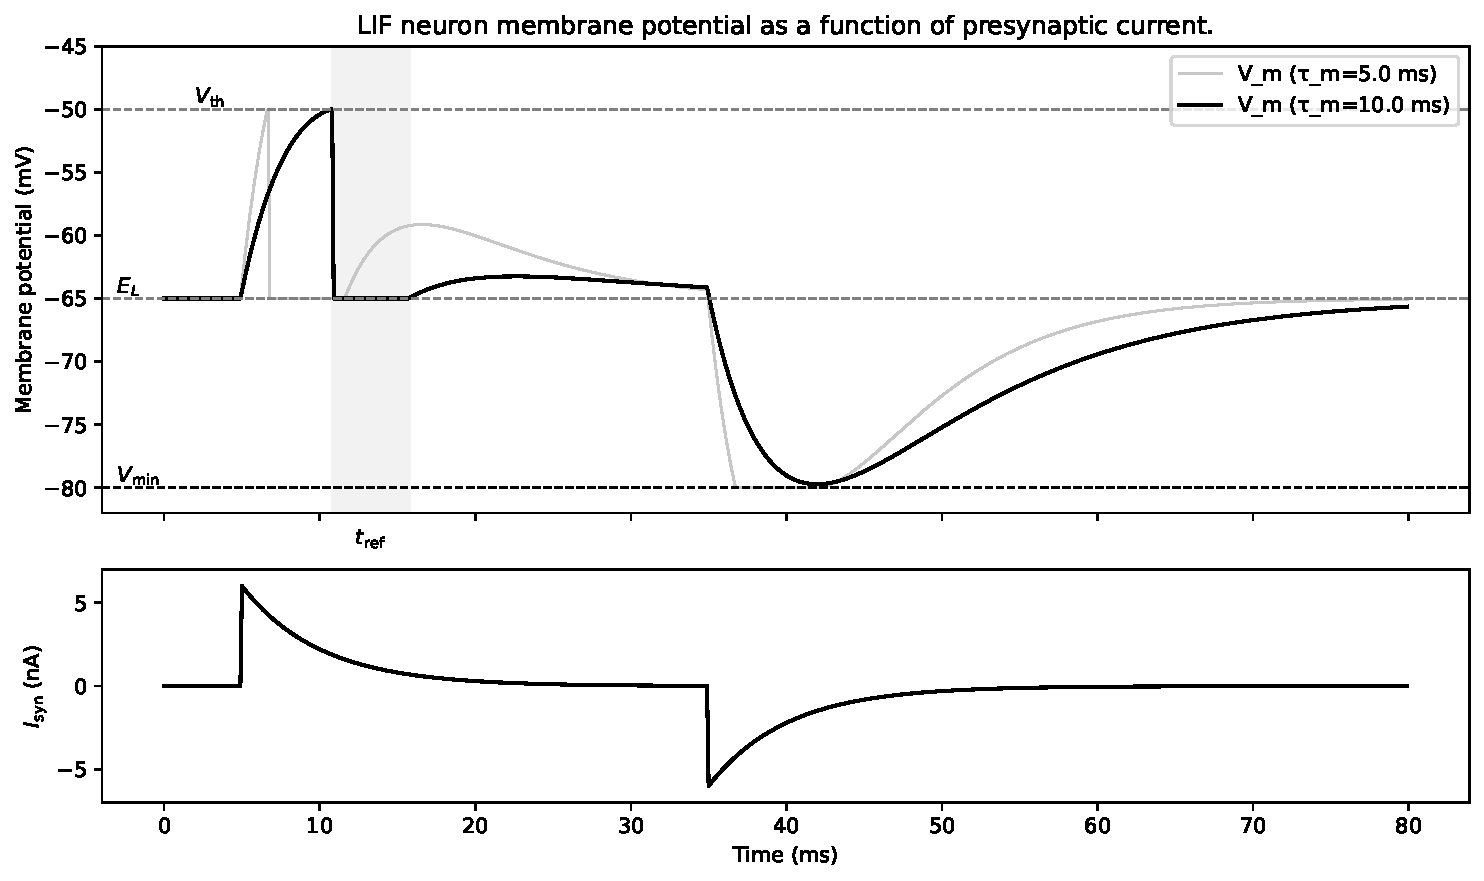
\includegraphics[width=1.0\textwidth]{neuron_models/mem_pot}
\end{center}
\caption{Change of membrane potential $V_m$ of an LIF neuron (\textit{leaky IAF}) as a function of presynaptic current $I_{\text{syn}}$ generated by two presynaptic neurons with exponential postsynaptic current: an excitatory neuron with weight $w_{\text{ex}}=6$ and an inhibitory neuron with weight $w_{\text{in}}=-6$. Other parameters are $\tau_{\text{syn, ex}} = \tau_{\text{syn, in}} = 5~\mathrm{ms}$, delay $d_j = 0~\mathrm{ms}$, $V_{\text{th}}=-50~\mathrm{mV}$, $E_L=-65~\mathrm{mV}$, $V_{\min}=-80~\mathrm{mV}$, $t_{\text{ref}}=5~\mathrm{ms}$, $I_e=0~\mathrm{nA}$, and $C_m=1~\mathrm{nF}$. Curves for $\tau_m=10~\mathrm{ms}$ and $\tau_m=5~\mathrm{ms}$ are shown to compare the influence of membrane time constant on dynamics. The excitatory neuron fires at $t=5~\mathrm{ms}$ and the inhibitory neuron at $t=35~\mathrm{ms}$.} 
\label{mem_pot}
\end{figure}

\newpage
\section{Model with an Exponential Kernel}
\label{eksponentno_jedro}
In the NEST simulator, which we will use to implement later systems, the exponential-kernel model (\textit{iaf\_psc\_exp}) is defined by a system of first-order differential equations (\citet{expModel}). The postsynaptic current $i(t)$ changes according to the system
\begin{align*}
    \frac{dx}{dt}&=\frac{z}{\tau_{rec}}-ux\delta({t-t_{sp}}) \\
    \frac{di}{dt}&=-\frac{i}{\tau_{\text{syn, X}}}+ux\delta({t-t_{sp}}) \\
    \frac{dz}{dt}&=\frac{i}{\tau_{\text{syn, X}}}-\frac{z}{\tau_{rec}} ,
\end{align*}
where $t_{sp}$ represents the presynaptic spike time, 
$\tau_{rec}$ the synaptic resource recovery time,
$u$ the fraction of synaptic resources consumed by a spike, and
$\delta(t-t_{sp})$ the delta distribution for instantaneous updates at spike times.
\\
\\
Let us verify whether the postsynaptic current after a spike indeed follows a simple exponential function. If we observe only the change of $i(t)$ over time without new spikes, then $\delta(t-t_{sp})=0$, and the differential equation for $i$ simplifies to
\begin{equation*}
    \frac{di}{dt}=-\frac{i}{\tau_{\text{syn, X}}} .
\end{equation*}
The solution of this differential equation is then
\begin{equation*}
    i(t)=i_0 e^{-t/\tau_{\text{syn, X}}} ,
\end{equation*}
where we see that the kernel is indeed an exponential function starting at $i_0$. The potential jump after a spike is scaled by synaptic weight $w$, therefore $i_0=w$, and the postsynaptic current is determined by the value of $\tau_{\text{syn, X}}$.

Now we can calculate the amount of charge transferred through the synapse after a spike. This will be useful for comparing and selecting an appropriate model for systems developed below (Section \ref{sec:izbira_modela}). The amount of charge $q$ transferred through the synapse after spike firing is defined
as the area under the postsynaptic current curve
\[
q = \int_0^{\infty} i_{\text{syn, X}}(t) dt = \tau_{\text{syn, X}} .
\]
\\
\noindent In the exponential kernel, postsynaptic current decay is determined by the constant $\tau_{\text{syn, ex}}$. At this value, the postsynaptic current reaches $36.8\%$ of the maximum value, while the alpha kernel reaches its maximum at this value, as shown in Figure \ref{neuron_psc}. The value of postsynaptic current for the exponential kernel at $t=\tau_{\text{syn, ex}}$ was calculated by the following equation.
\begin{align*}
    i_{\text{syn, ex}}(t) &= w e^{-\frac{t}{\tau_{\text{syn, ex}}}} \\
    i_{\text{syn, ex}}(\tau_{\text{syn, ex}}) &= w e^{-1} \approx 0.3679 w.
\end{align*}

\section{Model with an Alpha Kernel}
The alpha-kernel model is a more complex and biologically more realistic model of postsynaptic currents. In the NEST simulator, the postsynaptic current of the
alpha-kernel model (\textit{iaf\_psc\_alpha}) is defined as
\[
i_{\text{syn, X}}(t) = \frac{e}{\tau_{\text{syn, X}}} t e^{-\frac{t}{\tau_{\text{syn, X}}}} \Theta(t) ,
\]

where $\Theta(t)$ is the unit step function, which ensures that the postsynaptic current
is zero for times before spike firing.
The postsynaptic current is normalized so that it reaches a unit maximum at time
$t = \tau_{\text{syn, X}}$.

\[
i_{\text{syn, X}}(t = \tau_{\text{syn, X}}) = 1 .
\]
The equation describes the time course of postsynaptic current after firing of the
presynaptic neuron's action potential. The factor $t$ causes a gradual
rise of current after the spike, while the exponential term determines its later
decrease. Consequently, postsynaptic current does not reach maximum immediately at
spike firing, but only at time $\tau_{\text{syn, X}}$, which models the speed of
opening and closing of ion channels in biological synapses.

Parameter $\tau_{\text{syn, X}}$ determines the time scale of synaptic dynamics: a larger
value causes a slower rise and longer duration of postsynaptic current,
while a smaller one causes a faster and shorter response. This form of postsynaptic current leads to
smoother temporal integration of input spikes.

As with the exponential kernel, the total charge $q$ transferred by postsynaptic current in the alpha kernel is defined as the area under the postsynaptic current curve.
\[
q = \int_0^{\infty} i_{\text{syn, X}}(t) dt = e \tau_{\text{syn, X}} .
\]

\section{Choosing the Neuron Model}
\label{sec:izbira_modela}
In the systems implemented below, we try to use as few simplifications or generalizations as possible when modeling mechanisms in the human brain. For this purpose, the alpha-kernel neuron model is more suitable,
because it has a biologically more realistic shape of postsynaptic current. Nevertheless, both models are used below, because due to the different postsynaptic current shapes, the exponential-kernel model performs better for reinforcement learning.

For us, the most important difference is in the amount of transferred charge $q$. As described in Section \ref{sec:rstdp}, this affects how much external noise can influence spike frequency. The amount of transferred charge $q_{\text{alfa}}$ in the alpha kernel is greater than the transferred charge in the exponential kernel $q_{\text{exp}}$ by a factor $\frac{q_{\text{alfa}}}{q_{\text{exp}}} = e$. This difference can be adjusted with lower synaptic weights, while the difference in influence on spike frequency is due to the differently long time interval during which postsynaptic current is near its maximum value. In the alpha kernel this interval is longer than in the exponential kernel, so sequential postsynaptic spikes overlap much more over time. When integrating different postsynaptic currents over time, this creates a low-pass filter effect that smooths sudden changes in the amplitude of total current at the input of the postsynaptic neuron. If the neuron fires at a certain constant frequency, then with added noise the spike-frequency variance is lower for the alpha kernel than for the exponential one.
\\
\\
We compare frequency variance for both kernels over 5000 ms across five postsynaptic neurons, into which we independently inject Poisson noise. 

\subsubsection{Poisson Noise}
Poisson noise is formally described as a realization of a Poisson process, which is a stochastic process with discrete events in time. The Poisson process describes a sequence of spikes that appear independently of each other with a constant average rate of occurrence. If a Poisson process is observed in a finite time interval $\Delta t$, the number of spikes in that interval is distributed according to a Poisson distribution.

Let $N(t)$ be a Poisson process with parameter $\lambda$, where $N(t)$ denotes the total number of spikes up to time $t$. Then the probability that $k$ spikes occur in interval $\Delta t$ is given by
\begin{equation*}
    P(N(t + \Delta t) - N(t) = k) = \frac{(\lambda \Delta t)^k e^{-\lambda \Delta t}}{k!}, \quad k = 0, 1, 2, \ldots
\end{equation*}
Poisson noise in spiking neural networks represents sampling from a Poisson process, where each spike corresponds to one action potential. Such a model matches biological reality, since spikes in many neurons arise approximately independently and with variable interspike intervals. Parameter $\lambda$ determines the average firing frequency, while the stochasticity of the Poisson process causes variance in the number of spikes that equals the expected value, i.e., $E[N(\Delta t)] = Var(N(\Delta t)) = \lambda \Delta t$.

By injecting Poisson noise into postsynaptic neurons, we simulate realizations of a Poisson process that act as random synaptic inputs. This enables analysis of the spiking neural network response to a biologically plausible stochastic stimulus and comparison of firing-frequency stability and variance of different kernels.
\newpage
\noindent To achieve an approximately equal average number of postsynaptic neuron spikes for both compared kernels, synaptic weight between alpha-kernel neurons $w_{\text{alfa}}$ is by factor $e$ smaller than synaptic weights to exponential-kernel neurons $w_{\text{eksp}}$. All simulation parameters are listed in Table \ref{variance_simulation_parameters}. From simulation results shown in Table \ref{tab:isi_summary}, we observe the expected larger variance for the exponential kernel.

\begin{table}[htbp]
\centering
\begin{tabular}{ll}
\hline
\textbf{Parameter} & \textbf{Value} \\
\hline
Number of postsynaptic neurons & 5 \\
Simulation duration & 5000 ms \\
$C_m$ & 250.0 pF \\
$\tau_m$ & 20.0 ms \\
$E_L$ & 0.0 mV \\
$V_\text{th}$ & 20.0 mV \\
$V_\text{reset}$ & 0.0 mV \\
$t_\text{ref}$ & 2.0 ms \\
$\tau_\text{syn,ex}$ & 5.0 ms \\
$w_{\text{eksp}}$ & 25.0 \\
$w_{\text{alfa}}$ & 25.0 / $e \approx 9.20$ \\
Poisson noise frequency & 8000 Hz per neuron \\
\hline
\end{tabular}
\caption{Simulation parameters used for comparing neuron models.}
\label{variance_simulation_parameters}
\end{table}

\begin{table}[htbp]
\centering
\begin{tabular}{lcc}
\hline
Kernel & Mean (ms) & Variance (ms$^2$) \\
\hline
Exponential & \(7.846 \pm 0.021\) & \(\mathbf{0.402 \pm 0.028} \) \\
Alpha       & \(7.800 \pm 0.023\) & \(\mathbf{0.270 \pm 0.006} \) \\
\hline
\end{tabular}
\caption{Summary statistics of interspike intervals for neurons with alpha and exponential kernels. Mean and standard deviation are computed over all postsynaptic neurons.}
\label{tab:isi_summary}
\end{table}
\newpage
\section{R-STDP Synaptic Model}
\label{sec:synapse_model}
In the systems implemented in this thesis, we use a synapse with \textit{reward modulated spike timing dependent plasticity} (\textit{R-STDP}).
Spike timing dependent plasticity (\textit{STDP}) adjusts synaptic weights according to the relative timing of pre- and postsynaptic neuron spikes. In its classical form, STDP implements the \href{https://en.wikipedia.org/wiki/Hebbian_theory}{Hebbian principle}:
\begin{quote}
``Neurons that fire together, wire together.''
\end{quote}
To track ``co-firing'' of neuron pairs, we define an STDP value that represents the magnitude of potential synaptic-weight update between a neuron pair with respect to timing of pre- and postsynaptic spikes. In spiking neural networks, this enables tagging or strengthening synapses of neuron pairs that were responsible for firing of output neurons under stimulation of specific input neurons. This is called \textit{credit assignment}, which is one of the fundamental challenges in training spiking neural networks. In classical neural networks, gradient would be used for this purpose; in spiking neural networks, this role is played by the STDP value, which is positive if the presynaptic neuron fires before the postsynaptic one (\(\Delta t > 0\)), and negative if the presynaptic neuron fires after the postsynaptic one (\(\Delta t \leq 0\)). Thus STDP serves as a rough approximation of a gradient. Mathematically this is described by the STDP window function: 
\[
\mathrm{STDP}(\Delta t) =
\begin{cases}
A_+ e^{-|\Delta t|/\tau_+}, & \text{if } \Delta t > 0 \text{ (presynaptic before postsynaptic)} \\
A_- e^{-|\Delta t|/\tau_-}, & \text{if } \Delta t \le 0 \text{ (postsynaptic before presynaptic)}
\end{cases}
\]
\noindent where \(A_+\) and \(A_-\) are multipliers for potentiation and depression, and \(\tau_+\) and \(\tau_-\) are time constants that determine the influence window of timing differences.

Neuron pairs can be updated solely on the basis of $\mathrm{STDP}$ value, by which individual synapses are strengthened or weakened, but this value is usually used in combination with reward. The amount of reward or neuromodulator concentration for the entire spiking neural network or group of neurons modulates learning amplitude, i.e., connection updates. We therefore update the connection between a neuron pair according to STDP value and reward amount present at a given moment.

\subsection{Dopamine Modulation}
In all systems developed in this thesis, as the basis for a synapse that, in addition to STDP value, also accounts for reward, we use the R-STDP synapse model (\citet{distalReward}), where reward dependence is introduced via the neuromodulator dopamine. Dopamine concentration is often treated as a direct reflection of reward amount or state value in which the agent is located, but it modulates only synaptic plasticity, i.e., learning. Instead of implementing negative reward with negative dopamine concentration, which is a common approach, it is biologically more meaningful to achieve avoidance of undesirable states by learning actions that lead away from those states under positive dopamine concentration. Such a system is described in Section \ref{aversive}. 

In the R-STDP synapse, STDP value is tracked through the \emph{eligibility trace} \(c\), which increases for a given neuron pair at firing according to STDP value, and then decays over time according to parameter $\tau_c$. This enables assignment of responsibility even with delayed rewards, according to the difference between the time of neuron-pair activity and the time of delivered reward. Thus synapses that were active just before an increase in dopamine concentration will be treated (according to STDP value) as responsible for output-neuron activity that potentially caused the increase in dopamine concentration, i.e., reward. Synapses active further in the past are updated correspondingly less. Such learning is called \textit{three-factor learning}, which marks synapses for potential change and preserves information about past activity of pre- (first factor) and postsynaptic neurons (second factor) until the third factor arrives, in this case dopamine signal \(n\), representing dopamine concentration. This mechanism facilitates temporal credit assignment, since it enables linking fast neuronal activity with slower behavioral responses, so synapses receive an appropriate update even if reward or signal is delayed.

Compared with classical temporal-difference or TD algorithms in non-spiking neural networks, where eligibility traces are used to update states or actions in discrete time steps, in spiking neural networks eligibility trace \(c\) is directly tied to actual spike events and can be triggered at every interaction between pre- and postsynaptic neurons. Thus eligibility trace represents a local, biologically interpretable learning component consistent with experimental evidence for three-factor learning in the brain.

Dopamine concentration is represented by dopamine trace \(n\), which can be defined as a value that tracks activity of special dopaminergic neurons. With increased activity of dopaminergic neurons, dopamine trace increases; in the absence of activity, it decays according to parameter $\tau_n$. Dopamine trace is used for direct modulation of size and direction of synaptic plasticity, i.e., the magnitude and sign of connection-weight update. Synaptic dynamics of the R-STDP synapse is described by the following equations (\citet{dopamineSynapse}).
\[
\begin{aligned}
\dot{w} &= c \, (n - b), \\
\dot{c} &= -\frac{c}{\tau_c} + \mathrm{STDP}(\Delta t) \, \delta(t - s_{\text{pre/post}}) C_1, \\
\dot{n} &= -\frac{n}{\tau_n} + \frac{\delta(t - s_n)}{\tau_n} C_2.
\end{aligned}
\]
The equations describe dynamics of three key quantities: synaptic weight \(w\), eligibility trace \(c\), and dopamine trace \(n\). Synaptic weight \(w\) is updated directly as the product of current eligibility trace \(c\) and deviation of dopamine concentration \(n\) from basal value \(b\). Trace \(c\) tracks pairs of fired pre- and postsynaptic neurons and approximates responsibility of an individual synapse for firing of the postsynaptic neuron as a consequence of presynaptic activity. Its dynamics includes exponential decay with time constant \(\tau_c\) and impulse changes at each neuron firing, modulated by constant \(C_1\). Dopamine trace \(n\) decreases exponentially with its own time constant \(\tau_n\) and increases at dopaminergic-neuron firings occurring at times \(s_n\) and scaled by constant \(C_2\). Figure \ref{c_no_delay} shows changes of eligibility trace $c$ and synaptic weight $w$ as a function of pre- and postsynaptic neuron firing and dopamine trace $n$. Dopamine neurons that determine dopamine trace fire every 40 ms.
\begin{figure}[htbp]
\begin{center}
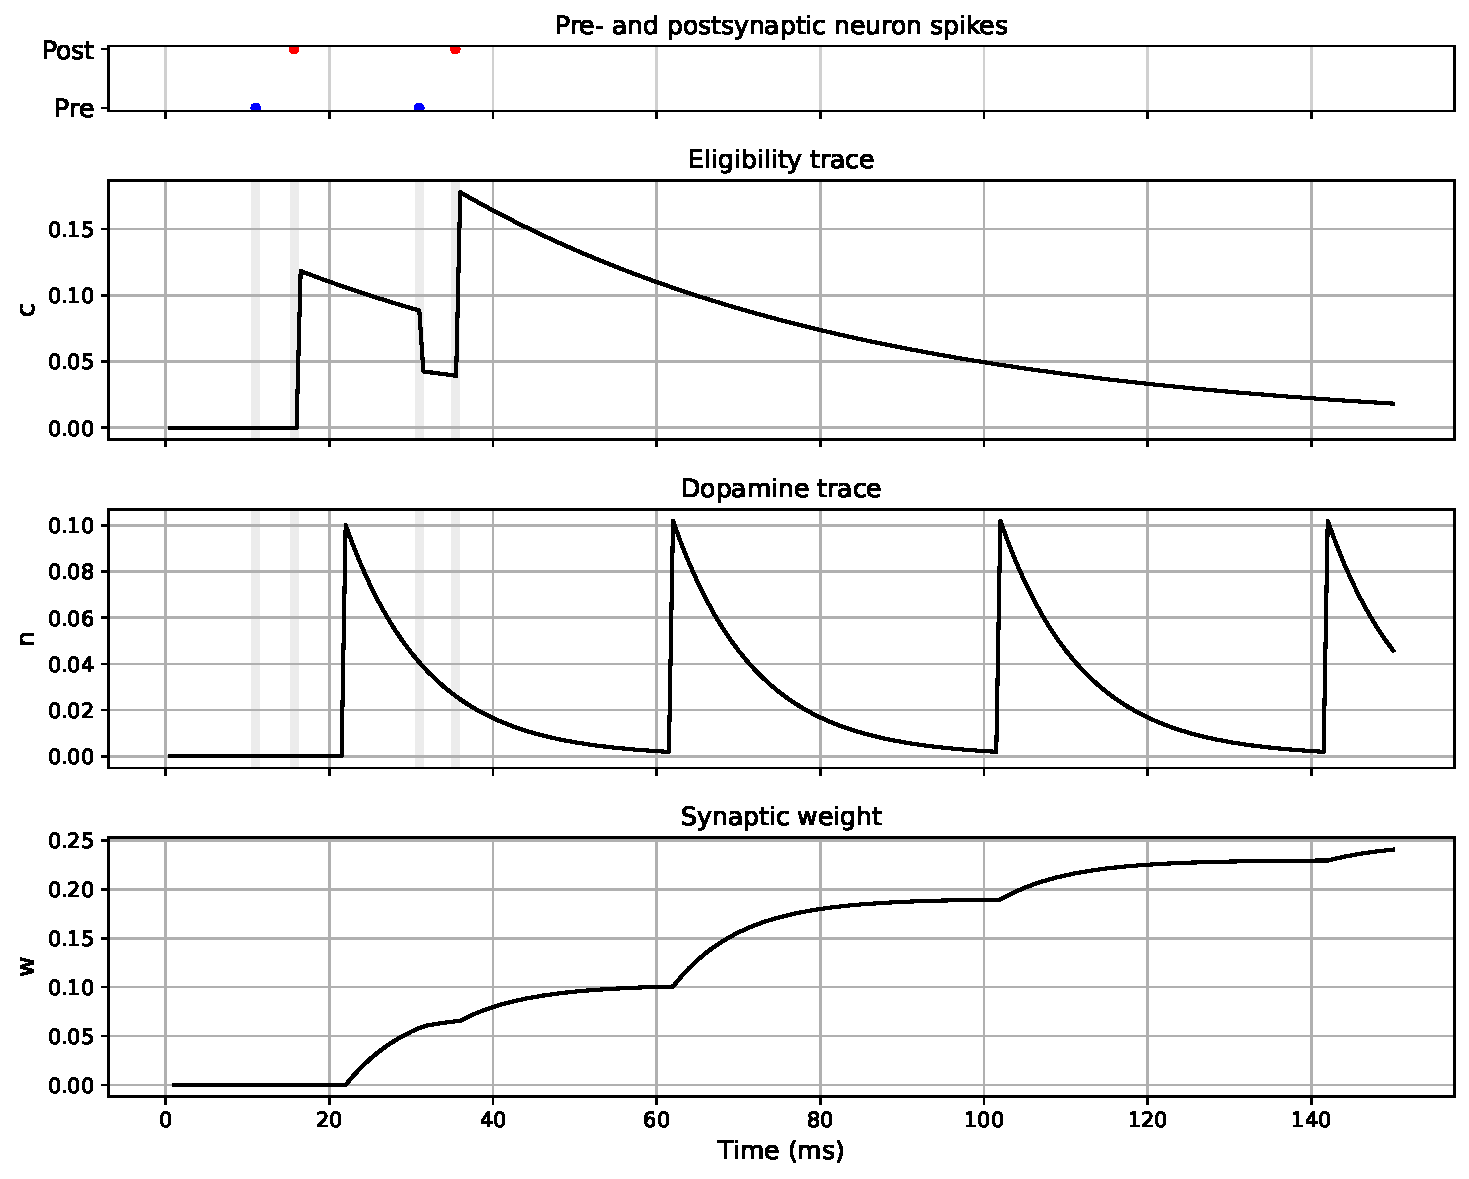
\includegraphics[width=0.9\textwidth]{neuron_models/RSTDP}
\end{center}
\caption{Eligibility trace $c$, dopamine trace $n$, and synaptic-weight changes for presynaptic spikes at $[10.0, 30.0]$ ms and postsynaptic spikes at $[12.0, 32.0]$ ms, simulated over $150$ ms with an R-STDP synapse and parameters $\tau_c = 50.0$ ms, $\tau_n = 10.0$ ms, $\tau_\mathrm{plus} = 10.0$ ms, $b = 0.0$, $A_\mathrm{plus} = 0.2$, $A_\mathrm{minus} = 0.2$, and synaptic delay $0.5$ ms. The figures show a positive eligibility trace due to presynaptic firing before postsynaptic firing. In the presence of non-zero dopamine trace $n$ at dopaminergic-neuron firing every 40 ms, synaptic weight $w$ is strengthened.}
\label{c_no_delay}
\end{figure}

\chapter{Reinforcement Learning on Spiking Neural Networks}
\label{sec:reinforcement_learning}
In this work, we use a classical reinforcement-learning agent that receives information about the external environment through stimulation of input neurons, and then as a response to the current state selects an action that affects the environment. If it reaches a rewarded state, we reward the agent. Through rewarding and interaction with the environment, the agent learns actions that in a given state lead to reward by updating connections that were active in the previous state and were responsible for the action that led us to the next state.

\section{R-STDP Learning}
\label{sec:rstdp}
R-STDP learning is based on strengthening connections that were responsible for the agent's correct action in a given state. We achieve this by increasing dopamine concentration across all connections, with strongest reinforcement on those connections that caused the largest number of postsynaptic neuron spikes as a direct consequence of presynaptic neuron firing. Such connections have the highest eligibility-trace value at reward arrival time.

Initially, our agent consists of $N_{in}$ input neurons representing possible states, connected to $N_a$ output neurons. Input and output are connected in an \textit{all-to-all} regime, where all input neurons are connected to output neurons. Upon entering a given state, the corresponding input neuron is stimulated so that it fires for $200$ ms at frequency $100$ Hz. The action is selected at the end of the interval based on activity of output neurons representing possible actions. Among them, we select the neuron that fired most often in the current state. If we enter a rewarded state, we stimulate $N_{\text{dopa}}$ dopamine neurons with current $600$ pA. At each spike, dopamine neurons uniformly project dopamine to all connections between input and output neurons.

With increased dopamine concentration upon entering a rewarded state, in addition to desired connections we might also update connections active in the new state. To avoid this, we disable updates for connections where reward arrived too quickly. We therefore adapt the R-STDP synapse by shifting the entire eligibility trace in time by $\tau_{c, \text{delay}}$, thereby preventing updates due to rewards that arrive in less than $\tau_{c, \text{delay}}$ after synapse activity. Dynamics of the adapted synapse is shown in Figure \ref{delayed_eligibility}.

\begin{figure}[htbp]
\begin{center}

\includegraphics[width=1.0\textwidth]{neuron_models/RSTDP_delayed}
\end{center}
\caption{Eligibility trace $c$, dopamine trace $n$, and synaptic-weight update for presynaptic spikes at $[10.0, 30.0]$ ms and postsynaptic spikes at $[12.0, 32.0]$ ms, simulated over $150$ ms with an R-STDP synapse using $\tau_c = 50.0$ ms, $\tau_{c,\mathrm{delay}} = 50.0$ ms, $\tau_n = 10.0$ ms, $\tau_\mathrm{plus} = 10.0$ ms, $b = 0.0$, $A_\mathrm{plus} = 0.2$, $A_\mathrm{minus} = 0.2$, and synaptic delay $0.5$ ms. The figure shows a positive eligibility trace due to presynaptic firing before postsynaptic firing, but shifted by $\tau_{c, \mathrm{delay}}=50$ ms. In the presence of non-zero dopamine trace $n$ at dopaminergic-neuron firing every 40 ms, synaptic weight $w$ is strengthened, but only after delay with respect to pre- and postsynaptic spikes. Thus, reward that arrives too quickly does not strengthen the synapse.}
\label{delayed_eligibility}
\end{figure}

Reward determined by dopamine-neuron activity is always greater than or equal to $0$, which means synapses only strengthen over time. Connections responsible for selecting a specific action in a specific state must therefore compete for dominance. In the presence of reward, we must strengthen connections responsible for selecting the correct action enough relative to others so that in the future they dominate other actions and increase probability of selecting the correct action. In our case, where dopamine concentration is the same for all connections at a given moment, the difference in update amplitude of individual connections is determined exclusively by eligibility traces.

Eligibility trace is higher for connections with higher weights, because such connections cause more postsynaptic spikes as a direct consequence of presynaptic neuron firing. At lower weight values, when all connections are approximately equal, a sufficiently large difference in eligibility trace is achieved through variance in spike frequency. This causes some synapses to contribute to an action slightly more or less by chance. This means eligibility-trace values differ among synapses, so dopamine modulation can update synapses differently and establish differentiation among them even if all connections have equal initial weights. At lower weight values, where deterministic synaptic contribution is not yet dominant, random spike variance serves as a mechanism that ``breaks symmetry'' and allows eligibility traces to differ until weights are large enough for deterministic contributions to dominate.

Differentiation between synapses is often achieved by allowing negative rewards, which negatively update synapses responsible for incorrectly selected actions. In our system we do not allow negative rewards, which require negative dopamine concentration, since negative dopamine concentration is not possible in nature. We therefore achieve spike-frequency variance with Poisson noise. In the differential equation governing change of $V_m$, at lower weight values external constant current $I_e$, generated in our case by a Poisson-noise generator, dominates over $I_{\text{syn}}$. Thus, until deterministic contribution of strengthened connections becomes dominant, Poisson noise has a greater effect on $V_m$, and spike-frequency variance is therefore higher.

This also serves as an \textit{exploration} mechanism, which at lower weights, when all connections have approximately equal weights, enables random action selection. During learning, as synapses strengthen, the agent selects actions mainly according to dominant synapses, which represents \textit{exploitation} of the learned policy (the probability of selecting an individual action in a given state). Our system will therefore gradually increase the ratio of exploitation to exploration over learning.

For the neuron model used below, we choose the exponential-kernel neuron model, since in this case Poisson noise causes higher output-neuron variance than the alpha-kernel model. This was shown in Section \ref{sec:izbira_modela}.

The main challenge for successful learning is selecting correct system hyperparameters that allow synapses to differentiate quickly enough. Since we do not allow negative rewards, all connections grow over time, which gradually reduces exploration and thus probability of selecting a random action. With unsuitable parameter choice, it can happen that all connections strengthen approximately uniformly until exploration is practically gone and action selection depends on a randomly dominant path from input neurons to output neurons. In what follows, we searched for suitable hyperparameters experimentally, with the most influential hyperparameters being frequency and weight of the connection from the Poisson-noise generator to output neurons, parameters $A_+$ and $A_-$, and parameter $\tau_c$.

\subsection{Simulator NEST}
In what follows, we implement all developed systems using the \href{https://www.nest-simulator.org/}{NEST} simulator. The backend and individual simulator components are implemented in C++, which enables efficient simulation of spiking neural networks. To use the delayed R-STDP synapse presented in previous sections, we must write a special C++ module for integration with other simulator components.
\\
\\
To start, we implement R-STDP learning on a simple task with three states, numbered 0, 1, and 2. In each state, the agent can choose action 0, 1, or 2. Transition to a state after action selection is random (independent of chosen action), and in each state only one action choice is rewarded. In state 0, represented by stimulation of input neuron 0, we select action 0, represented by output neuron 0, as rewarded; in state 1 action 1, and in state 2 action 2. Figure \ref{rstdp_simple} shows dominance of correct synapses, increase of synaptic divergence over time, and growth of reward frequency during learning. In simulation, we use default NEST parameters for exponential-kernel neurons (\textit{iaf\_psc\_exp}) and delayed dopamine-modulated synapses. Other system parameters are listed in Table \ref{tab:rstdp_simple}.
 
\begin{table}[htbp]
\begin{tabular}{lll}
\textbf{Symbol} & \textbf{Meaning} & \textbf{Value} \\ \hline
$t_{\text{SIM}}$ & Simulation duration & 60000 ms \\ \hline
$w_{\text{motor, min}}$ & \makecell[l]{Minimum synaptic weight \\ between input and \\ output neurons} & 500 \\ \hline
$w_{\text{motor, max}}$ & \makecell[l]{Maximum synaptic weight \\ between input and \\ output neurons} & 2000 \\ \hline
$\tau_c$ & & 5 ms \\ \hline
$\tau_{c,\mathrm{delay}}$ & & 200 ms \\ \hline
$\tau_n$ & Dopamine-trace decay & 10 ms \\ \hline
$\tau_+ = \tau_-$ & Positive STDP constant & 20 ms \\ \hline
$b$ & \makecell[l]{Basal dopamine \\ concentration} & 0.1 \\ \hline
$A_+$ & Positive STDP multiplier & 0.7 \\ \hline
$A_-$ & Negative STDP multiplier & 0.3 \\ \hline
$d$ & Synaptic delay & 0.5 ms \\ \hline
$\lambda_{\text{motor}}$ & \makecell[l]{Average Poisson \\ noise rate} & 1000 Hz \\ \hline
$w_{\text{Poisson}}$ & Poisson-noise synaptic weights & 100 \\  \hline
$w_{\text{init, motor}}$ & \makecell[l]{Initial synaptic weights \\ between input and output \\ neurons} & $w_{\text{init, motor}} \sim \mathcal{N}(1300, 1)$ \\ \hline
\end{tabular}
\caption{Simulation parameters for R-STDP learning on a simple problem.}
\label{tab:rstdp_simple}
\end{table}

\begin{figure}[htbp]
\begin{center}

\includegraphics[width=1.0\textwidth]{rstdp/competition}
\end{center}
\caption{Display of synaptic weights between input and output neurons and average activity of dopaminergic neurons during simulation of R-STDP learning on a simple problem. From the weights, it is clear that synapses between input and output neurons representing the correct action gradually dominate other actions. Consequently, the frequency of selecting the correct action in each state increases, which is visible in the graph of average dopaminergic-neuron activity becoming increasingly ``denser''.} 
\label{rstdp_simple}
\end{figure}
\newpage
\subsection{Pong Game}
In the following, we present R-STDP learning on a more complex problem: the game \href{https://en.wikipedia.org/wiki/Pong}{\textit{Pong}}. R-STDP learning is short-sighted, since we learn actions only if reward follows immediately, but not if reward is delayed. For delayed rewards, TD (\textit{Temporal Difference}) learning can be used, which we implement in Section \ref{sec:td_learning}; for now, however, we map playing Pong, which normally requires prediction and has delayed reward, to a problem with immediate rewards. We define the game such that the ball has constant speed, given direction, and position in the $(x, y)$ plane. On one side of the field, our agent moves a paddle horizontally; on the other side is a wall from which the ball bounces elastically. This configuration is shown in Figure \ref{pong_setup}. If prediction were required from the agent, states would need to be defined as the Cartesian product of ball position $(x, y)$, its direction, and paddle $x$ position. We simplify the problem into a ball-tracking problem, as in \citet{pilotStudy}, where the agent chooses the desired target point of the paddle. Prediction is therefore not required. Both agent states and actions are discretized possible ball $x$ positions. The state is rewarded by stimulation of dopaminergic neurons with current $I_{R}$, which is proportional to the difference between reward $R_b$, calculated from distance between desired position $j$ and current ball $x$ position $k$, and average reward $\bar{R}_i$ at iteration $i$. With average reward, we limit synaptic strengthening if it does not improve the current policy.

\begin{align*}
R_b &= \begin{cases}
    1-|j-k| \cdot 0.3 & \text{if} \ |j-k|\leq3, \\
    0 & \text{otherwise}.
    \end{cases} \\
I_{R} &= \max(R_b-\bar{R}_i, 0) \cdot 600 \text{ pA}
\end{align*}

\begin{figure}[htbp]
\begin{center}

\includegraphics[width=0.5\textwidth]{figures/pong_setup}
\end{center}
\caption{Graphical presentation of the agent and environment (\citet{pilotStudy}).}
\label{pong_setup}
\end{figure}
\newpage
We expect that in individual states, synapses leading from the input neuron to actions around the output neuron representing the same current ball $x$ position will dominate. We discretized the field along the $x$ axis into 20 states. After a simulation lasting 4000 iterations (ball positions) of 200 ms each, Figure \ref{rstdp_pong_learning} shows a graph of connections between the input neuron representing position $x=5$ and 20 output neurons, where output neuron 5 dominates during learning, followed by output neuron 4. For simulation, we used the same parameters as in the R-STDP learning example on a simple problem.

\begin{figure}[htbp]
\begin{center}

\includegraphics[width=1.0\textwidth]{rstdp/rstdp-pong/learning}
\end{center}
\caption{Graph of connection weights between input neuron 5 and output neurons during simulation of 4000 iterations (ball positions) of 200 ms each in Pong gameplay. During learning, the connection to output neuron 5 expectedly dominates, which represents tracking the ball.}
\label{rstdp_pong_learning}
\end{figure}
\newpage
\subsubsection{Results}
\subsubsection{Results}
We track learning using average survival time, which represents the time elapsed since the last missed ball or game start. Average survival time is calculated from the sequence of times between individual missed ball returns. At each iteration, time since the last missed return is increased by simulation step length (200 ms), and reset to zero at a miss. This gives a survival-time sequence showing how long the agent successfully returns the ball between two consecutive errors. Average survival time is then determined as the cumulative mean of these values over time, which means that at each time point we consider the mean of all survival times measured up to that point. We expect the shape of the total average reward curve to follow the average survival time curve, since successful ball tracking gives the agent higher and more frequent rewards. For scaled values of average reward and average survival time, Figure \ref{mean_reward} shows that the two curves have similar shape and both increase over time. Because average reward directly reflects selection of correct actions in a given state, with a properly defined reward function for an arbitrary problem, learning quality can be monitored using only total average reward.
\begin{figure}[htbp]
\begin{center}

\includegraphics[width=1.0\textwidth]{rstdp/rstdp-pong/mean_reward}
\end{center}
\caption{Total average reward $\bar{R}_i$ and average survival time over 4000 iterations of 200 ms. With aligned ranges of both values, it is evident that the curves have approximately the same shape and both rise over time.}
\label{mean_reward}
\end{figure}
\\
\\
R-STDP learning in this form is effective only for non-distant rewards, or in other words, the agent will not learn a potential path through different unrewarded states to reach the final reward. An example of a delayed-reward problem is searching for a path to reward in a grid, where the agent can move to neighboring cells left, right, up, and down. In the current implementation, the agent learns transitions only from states directly adjacent to the rewarded state.

During learning, we reward the agent when it transitions to the terminal state, then place it in a random state. We visualize the final agent policy by showing the preferred direction in each grid cell $i$. Probability of selecting an individual action is approximated by average connection weight from input to output neuron. Preferred direction for individual state $i$ is shown by normalized vector $\hat{x}_i$. We expect vectors of states directly adjacent to the goal to point toward the goal.
\[
\begin{aligned}
    \overrightarrow{x_i} &= \sum_{j=0}^{3} w_{ij} \cdot \overrightarrow{d}_j, \\
    L_i &= ||\overrightarrow{x_i}||, \\
    \hat{x}_i &= \begin{cases} \frac{\overrightarrow{x_i}}{L_i} & \text{if } L_i > 0 \\
        0 & \text{otherwise}
    \end{cases},
\end{aligned}
\]

\noindent
where \(w_{ij}\) is the synaptic weight from input neuron \(i\) to output neuron \(j\), and $\overrightarrow{d}_j$ is the direction vector representing action of output neuron \(j\):
\[
\overrightarrow{d}_0 = (0,1), \quad
\overrightarrow{d}_1 = (0,-1), \quad
\overrightarrow{d}_2 = (-1,0), \quad
\overrightarrow{d}_3 = (1,0).
\]
\\
An additional indicator of learning the correct action in state $i$ is the maximum difference between weights from input neuron $i$ to each output neuron, which approximates action-selection probability. For a good policy, we want probability of selecting the correct action to be appropriately larger than others. In R-STDP learning as implemented so far, we expect noticeable action differentiation in states directly adjacent to the goal, while for other states we expect the maximum weight difference to be minimal, since in those states we do not provide reward that would encourage learning. State vectors and maximum weight differences are shown via cell color in Figure \ref{rstdp_3x3}. The figure shows policy after learning for 500 iterations on a $4 \times 4$ grid and confirms expected results, where only cells directly adjacent to the goal have large maximum weight difference and correct vector direction. The result confirms that the agent is not able to learn a path to reward from an arbitrary state, but only from states directly adjacent to reward.

\begin{figure}[htbp]
\begin{center}

\includegraphics[width=0.6\textwidth]{rstdp/rstdp-gridworld/best}
\end{center}
\caption{Visualization of the model policy on a $4 \times 4$ grid after 500 iterations of 200 ms. The terminal state is colored green. Color of other states shows the maximum difference between weights from the input neuron representing that state and individual output neurons representing actions. In each cell, an arrow shows the preferred action vector (direction) according to weights between the input neuron and individual output neurons. We see that only cells directly adjacent to the goal are brightly colored (have a large maximum difference among weights representing individual actions). Similarly, only these cells have correctly oriented vectors.}
\label{rstdp_3x3}
\end{figure}

\newpage
\section{TD Learning and the Actor-Critic Model}
\label{sec:td_learning}
Temporal Difference Learning (\textit{TD}) is a reinforcement-learning method that updates estimates of state values or state-action pairs online, during direct interaction with the environment. The key advantage of TD learning is its ability to learn from delayed rewards, since it enables gradual propagation of reward information back through a sequence of preceding states. Instead of waiting for the final outcome of an episode (the sequence of state transitions until reaching terminal state), TD learning compares the current value estimate with the so-called TD error $\delta_t$, based on the next state and possible immediate reward. In this way, actions that do not themselves bring immediate reward but lead to later success are also appropriately evaluated over time.
\\
\\
\noindent The basic update equation for the state-value function:
\[
V(s_t) \leftarrow V(s_t) + \alpha\,\delta_t,
\]

\noindent where \(\alpha\) is the learning rate, and TD error \(\delta_t\) is defined as

\[
\delta_t = r_{t+1} + \gamma V(s_{t+1}) - V(s_t).
\]
\noindent In the expression, \(r_{t+1}\) is reward at transition from state \(s_t\) to state \(s_{t+1}\), and factor \(\gamma \in [0,1]\) determines relative weight of future rewards. TD error represents the difference between the improved value prediction and previous estimate.
\\
\\
\noindent In this work, we implement the TD(0) algorithm, where values are updated exclusively on the basis of current reward and estimated value of the next state. Action selection in each state is rewarded using the same R-STDP mechanism as before, with synapses updated using eligibility traces. This actually also makes it possible to reward synapses representing action choices from states further in the past, which is the idea of the more general TD-learning form, TD($\lambda$). If we define states with a longer stimulation interval of the input neuron and appropriately choose constant $\tau_c$, which determines eligibility-trace decay, we achieve minimal influence of synapses that do not represent action choice in the current state, and thus approximate TD(0). This greatly facilitates monitoring learning and searching for suitable hyperparameters, which can otherwise be demanding in spiking neural networks.

\subsection{Actor-Critic Model}
For TD learning, in addition to the already developed R-STDP module for learning correct action selection, we also need a module that computes TD error $\delta_t$. Such a model is called \textit{actor-critic}. In this thesis, we aim for implementations that are as biologically plausible as possible, therefore we want the spiking neural network itself to compute TD error. For this, we follow \href{https://en.wikipedia.org/wiki/Basal_ganglia}{basal ganglia}, shown in Figure \ref{basal_ganglia}, a group of neurons in the human brain that, among other things, realizes a form of TD learning. To simplify and abstract the complex system and mechanisms present in real basal ganglia, we follow \citet{actorCritic}. The goal of the system developed below is, on a grid task, to achieve delayed-reward propagation to states that gradually lead to the goal, and thus learn an optimal policy for navigating to reward.
\begin{figure}[htbp]
\begin{center}
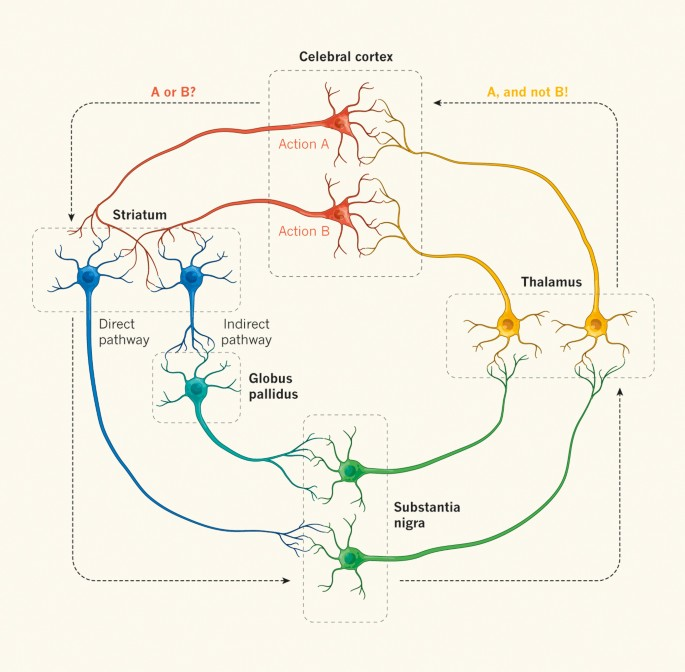
\includegraphics[width=0.6\textwidth]{figures/basal_ganglia}
\end{center}
\caption{Diagram of basal-ganglia neuron groups (\citet{bazal}).}
\label{basal_ganglia}
\end{figure}
\newpage
As mentioned, the actor-critic model presented by \citet{actorCritic} is a simplification and abstraction of real mechanisms in the brain that enable this. In basal ganglia, as shown in Figure \ref{basal_ganglia}, several neuron groups and connections participate, which in this model are logically merged into \textit{cortex}, representing input neurons, \textit{motor neurons}, representing output neurons and possible actions, and critic neuron groups: \textit{striatum}, \textit{ventral pallidum}, and dopaminergic neurons. \textit{Substantia nigra} and \textit{thalamus} of real basal ganglia are functionally merged into dopaminergic neurons that project dopamine to connections between input and striatum and between input and output motor neurons.
Both in basal ganglia and in the actor-critic model by Wiebke P. et al., we distinguish two main pathways: \textit{direct} and \textit{indirect}, leading from striatum neurons to dopaminergic neurons. The direct pathway is a delayed inhibitory pathway running directly from striatum to dopaminergic neurons,
while the indirect pathway is inhibitory to ventral-pallidum neurons, a special neuron group that inhibits dopaminergic-neuron activity. Ventral pallidum is located ventral to \textit{globus pallidus}, shown in classical basal-ganglia diagrams, and is associated with reward expectation and decision-making, so Wiebke P. et al. likely chose this naming for the indirect-pathway neuron group. The described actor-critic model is shown in Figure \ref{actor-critic}.
\begin{figure}[htbp]
\begin{center}
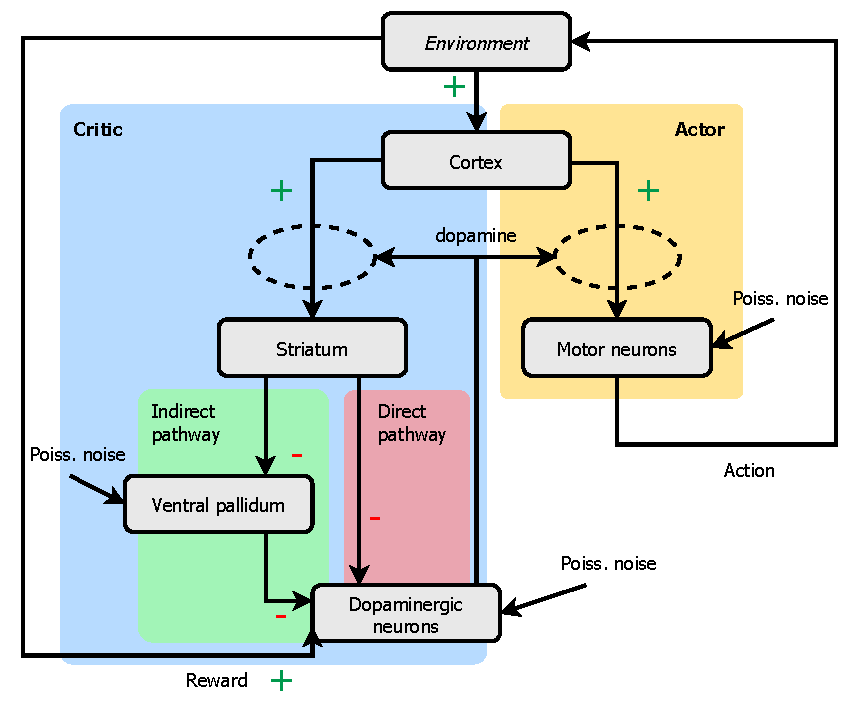
\includegraphics[width=1.0\textwidth]{figures/actor-critic}
\end{center}
\caption{Actor-critic model as proposed by \citet{actorCritic}.}
\label{actor-critic}
\end{figure}

\noindent In the presence of a basic, constantly present non-zero frequency of ventral-pallidum neurons, induced by injected Poisson noise, activity of the indirect pathway has an excitatory effect on dopaminergic neurons. Activity of ventral-pallidum neurons lowers activity of dopaminergic neurons through an inhibitory connection. If, through an inhibitory connection from striatum, we reduce ventral-pallidum neuron activity, dopaminergic-neuron activity rises. Indirect and direct connections to dopaminergic neurons act competitively. Synapses in the indirect pathway have minimal delay due to signal transmission. Thus, the indirect pathway maps increased striatum activity in the current state, with minimal delay, into increased dopaminergic-neuron activity. At the same time, during time spent in the current state, the direct connection inhibits dopaminergic neurons proportionally to striatum activity, but according to its activity in the previous state, since the direct pathway is delayed. Together, indirect and direct connections compute TD error $\delta_t$, which in the current state, according to the computed approximation of current-state value, strengthens synapses of the previous state that were responsible for selecting the action that brought us to the current state.

This mechanism is shown in Figure \ref{actor_critic_learning}. The average synaptic weight between input neuron $i$ and striatum represents expected reward and an approximation of state value $i$. When transitioning from a state with high average weight of synapses to striatum to a state with low average weight, the direct connection dominates and dopaminergic neurons are inhibited, and vice versa. If we move to a state with approximately equal average connection weight to striatum, direct and indirect connections cancel out, and dopaminergic neurons fire at a frequency determined by external Poisson noise.

\subsubsection{Implementation}
The group of input neurons, i.e., cortex, is represented by $N_{\text{in}}$ neurons connected to $N_a$ motor (output) neurons. In the actor, for reasons given in Section \ref{sec:rstdp}, we use the exponential-kernel neuron model; in the critic, biologically more realistic alpha-kernel neurons are used. Since input neurons are shared by actor and critic, we add an extra level of $N_{\text{in}}$ input motor neurons between input and output neurons, connected with input neurons via static connections with weights $w_{\text{in}\to\text{in, motor}}$ in \textit{one-to-one} regime, i.e., one input neuron to one intermediate-level neuron. This intermediate level allows tuning frequency and noise needed for R-STDP learning in the actor separately from the critic, which facilitates search for suitable hyperparameters. Intermediate neurons are connected to output neurons in \textit{all-to-all} regime (each input neuron connected to each output neuron) via delayed R-STDP synapses with normally distributed weights. Input neurons are also connected in \textit{all-to-all} regime to $N_{\text{critic}}$ striatum neurons via delayed R-STDP synapses with normally distributed weights. Striatum is connected via static inhibitory connections with weights $w_{\text{str}\to\text{vp}}$ to $N_{\text{critic}}$ ventral-pallidum neurons, and via static inhibitory connections with weights $w_{\text{str}\to\text{dopa}}$ and delay $d_{\text{dir}}$ to $N_{\text{dopa}}$ dopaminergic neurons.
Ventral pallidum is also connected to dopaminergic neurons through static inhibitory connections that are not delayed and have weights $w_{\text{vp}\to\text{dopa}}$. All critic connections use \textit{all-to-all} regime. Poisson noise with average rate $\lambda_{\text{in, motor}}$ is injected into intermediate-level neurons between input and output neurons, and Poisson noise with rate $\lambda_{\text{out, motor}}$ is injected into output neurons. Poisson noise is also injected into ventral-pallidum neurons with average rate $\lambda_{\text{vp}}$ and into dopaminergic neurons with average rate $\lambda_{\text{dopa}}$.
Poisson-noise generators are connected to individual neuron groups through static connections with weights $w_{\text{ext, in}}$, $w_{\text{ext, out}}$, $w_{\text{ext, vp}}$, and $w_{\text{ext, dopa}}$. Hyperparameters of R-STDP synapses and neuron models, together with other hyperparameters, are listed in Section \ref{sec:izbira_parametrov}. The described model is shown in Figure \ref{actor_critic_diagram}.
\begin{figure}[htbp]
\begin{center}

\includegraphics[width=1.0\textwidth]{figures/dipl_TD_model}
\end{center}
\caption{Visualization of the implemented actor-critic system, where at iteration $i$ the environment signals state $s_i$ to the system by stimulating the corresponding input neuron. The actor selects action $a_i$, and on transition to a new state the environment stimulates dopaminergic neurons with current $I_{R, i-1}$, representing potential reward.}
\label{actor_critic_diagram}
\end{figure}

Unlike the original system (\citet{actorCritic}), for the synapse model we use our delayed R-STDP synapse, developed in Sections \ref{sec:synapse_model} and \ref{sec:rstdp}, which in addition to presynaptic spikes also accounts for postsynaptic spikes according to STDP rule. This allows us to use as the actor the R-STDP system developed in Section \ref{sec:rstdp}. Our implementation also differs in action-selection method: for selected action, we choose the one whose corresponding output neuron has the highest spike count in the current state. In the original system, action is selected according to the first spike of the corresponding output neuron fired as a result of stimulation in the current state. With this method, after the first spike we must inhibit all other output neurons in as short a time interval as possible. This directly strengthens connections responsible for selected activity, since inhibition yields zero eligibility traces for synapses to other output neurons, because they do not fire. In this case there is also no need for synaptic competition, but we must therefore check output-neuron spikes at every simulator step. In NEST, this is every 0.1 ms, which is problematic because the simulator runs in C++ backend that we exit immediately when simulation is interrupted. Thus there is an essential difference between running \texttt{nest.Simulate(0.1)} 100 times or \texttt{nest.Simulate(10)} once. Due to simulation speed, our system is smaller in number of neurons than the original system.

\subsection{Parameter Selection}
\label{sec:izbira_parametrov}
Parameters were selected experimentally, this time without considering biological accuracy. When changing sizes of individual neuron groups, in parameter selection we must ensure preserving baseline frequency of dopaminergic neurons and balance between inhibition and excitation due to direct and indirect connections. Reduction of frequency performed by the neuron layer between input and output neurons must be large enough so that noise at baseline synaptic weights between the middle layer and output neurons enables learning, as explained in Section \ref{sec:rstdp}.
Tables \ref{tab:params1}-\ref{tab:params6} list constants and parameters of the implemented model. Parameters not shown in tables have default values of the NEST simulator.

\begin{table}[htbp]
\begin{tabular}{lll}
\textbf{Symbol} & \textbf{Meaning} & \textbf{Value} \\ \hline
% ------- Simulation constants -------
%TODO: number of neurons
POLL\_TIME & Simulation time per iteration & 200 \\ \hline
\(f(s_{\text{in}, i})\) & stimulation frequency of input neuron $i$ & $100$ Hz \\ \hline
%\(n_{\text{kritik}}\) & Število nevronov v skupinah nevronov kritika & 8 \\ \hline
\end{tabular}
\caption{Simulation parameters}
\label{tab:params1}
\end{table}
\begin{table}[htbp]
\begin{tabular}{lll}
\textbf{Symbol} & \textbf{Meaning} & \textbf{Value} \\ \hline
\thead[l]{\bfseries Critic neuron \\
\bfseries group parameters} \\
type & Neuron model type & \textit{iaf\_psc\_alpha} \\ \hline
\(C_{m,\text{in}}\) & Membrane capacitance & 250.0 pF \\ \hline
\(\tau_{m,\text{in}}\) & Membrane time constant & 10.0 ms \\ \hline
\(V_{\text{reset,in}}\) & Reset potential & 0.0 mV \\ \hline
\(V_{\text{th,in}}\) & Firing threshold & 20.0 mV \\ \hline
\(t_{\text{ref,in}}\) & Refractory period & 0.5 ms \\ \hline
\(\tau_{\text{syn,ex,in}}=\tau_{\text{syn,in,in}}\) & \makecell[l]{Excitatory and inhibitory \\ synaptic constant} & 2 ms \\ \hline
\(\tau_{\text{-,a}}\) & Negative STDP constant & 20.0 ms \\ \hline
\(V_{m,\text{in}}\) & Initial membrane potential & 0.0 mV \\ \hline
\(E_{L,\text{in}}\) & Resting potential & 0.0 mV \\ \hline
\\
\thead[l]{\bfseries Motor-neuron \\
\bfseries parameters} \\
type & Neuron model type & \textit{iaf\_psc\_exp} \\ \hline
\(C_{m,a}\) & \makecell[l]{Membrane capacitance \\ of motor neurons} & 250.0 pF \\ \hline
\(\tau_{m,a}\) & Membrane time constant & 10.0 ms \\ \hline
\(V_{\text{reset,a}}\) & Reset potential & 0.0 mV \\ \hline
\(V_{\text{th,a}}\) & Firing threshold & 20.0 mV \\ \hline
\(t_{\text{ref,a}}\) & Refractory period & 0.1 ms \\ \hline
\(\tau_{\text{syn,ex,a}}=\tau_{\text{syn,in,a}}\) & \makecell[l]{Excitatory and inhibitory \\ synaptic constant} & 2 ms \\ \hline
\(\tau_{\text{-,a}}\) & Negative STDP constant & 20.0 ms \\ \hline
\(V_{m,a}\) & Initial membrane potential & 0.0 mV \\ \hline
\(E_{L,a}\) & Resting potential & 0.0 mV \\ \hline
\end{tabular}
\caption{Neuron parameters}
\label{tab:params2}
\end{table}

\begin{table}[htbp]
\begin{tabular}{lll}
\textbf{Symbol} & \textbf{Meaning} & \textbf{Value} \\ \hline
\\
\thead[l]{\bfseries Synapse parameters between \\
\bfseries input and \\
\bfseries input motor \\
\bfseries neurons} \\ \hline
type & Synapse type & \makecell[l]{Default \\ constant \\ NEST synapse} \\ \hline
\(w_{\text{in}\to\text{in, motor}}\) & \makecell[l]{Synaptic weights between \\ input and input \\ motor neurons} & 120 \\ \hline
\\
\thead[l]{\bfseries Synapse parameters between \\
\bfseries input and \\
\bfseries output motor \\
\bfseries neurons} \\ \hline
% ------- STDP parameters (delayed_synapse) -------
type & Synapse type & \makecell[l]{Delayed \\ R-STDP synapse} \\ \hline
\(\tau_{c}\) & Eligibility-trace decay & 5 ms \\ \hline
\(\tau_{c\text{, delay}}\) & Delay of trace $c$ & 200 ms \\ \hline
\(\tau_{n}\) & Dopamine-trace decay & 10 ms \\ \hline
\(\tau_{+}\) & Positive STDP constant & 20 ms \\ \hline
\(b\) & \makecell[l]{Basal dopamine \\ concentration} & 0.1  \\ \hline
\(A_{+}\) & Positive STDP multiplier & 1.5 \\ \hline
\(A_{-}\) & Negative STDP multiplier & 1.0 \\ \hline
\(W_{\min,a}\) & Minimum weight & 500 \\ \hline
\(W_{\max,a}\) & Maximum weight & 4000 \\ \hline
\(w_{\text{in, motor}\to a}\) & \makecell[l]{Initial synaptic weights between \\ input and output \\ motor neurons} & \(\mathcal{N}(1300, 1)\) \\ \hline
\end{tabular}
\caption{Synapse parameters between input and motor neurons}
\label{tab:params3}
\end{table}
\begin{table}[htbp]
\begin{tabular}{lll}
\textbf{Symbol} & \textbf{Meaning} & \textbf{Value} \\ \hline
\thead[l]{\bfseries Synapse parameters between \\
\bfseries input neurons \\
\bfseries and striatum} \\ \hline
% ------- STDP parameters (delayed_synapse) -------
type & Synapse type & \makecell[l]{Delayed \\ R-STDP synapse} \\ \hline
\(\tau_{c}\) & Eligibility-trace decay & 5 ms \\ \hline
\(\tau_{c\text{, delay}}\) & Delay of trace $c$ & 200 ms \\ \hline
\(\tau_{n}\) & Dopamine-trace decay & 10 ms \\ \hline
\(\tau_{+}\) & Positive STDP constant & 20 ms \\ \hline
\(b\) & \makecell[l]{Basal dopamine \\ concentration} & 0.1  \\ \hline
\(A_{+}\) & Positive STDP multiplier & 1.5 \\ \hline
\(A_{-}\) & Negative STDP multiplier & 1.0 \\ \hline
\(W_{\min,str}\) & Minimum weight & 150 \\ \hline
\(W_{\max,str}\) & Maximum weight & 1000 \\ \hline
\(w_{\text{in}\to \text{str}}\) & \makecell[l]{Initial synaptic weights between \\ input and striatum neurons} & \(\mathcal{N}(150, 8)\) \\ \hline
\end{tabular}
\caption{Synapse parameters between input and striatum}
\label{tab:params4}
\end{table}
\begin{table}[htbp]
\begin{tabular}{lll}
\textbf{Symbol} & \textbf{Meaning} & \textbf{Value} \\ \hline
type & Synapse type & \makecell[l]{Default constant \\ NEST synapse} \\ \hline
\(w_{\text{str}\to\text{vp}}\) & \makecell[l]{Synaptic weights between striatum \\ and ventral pallidum} & -50 \\ \hline
\(w_{\text{str}\to\text{dopa}}\) & \makecell[l]{Synaptic weights between striatum \\ and dopaminergic neurons} & -55 \\ \hline
\(w_{\text{vp}\to\text{dopa}}\) & \makecell[l]{Synaptic weights between \\ ventral pallidum and \\ dopaminergic neurons} & -65 \\ \hline
\(d_{\text{dir}}\) & \makecell[l]{Synaptic delay of \\ direct pathway} & 200 ms \\ \hline
\end{tabular}
\caption{Critic synapse parameters}
\label{tab:params5}
\end{table}
\begin{table}[htbp]
\begin{tabular}{lll}
\textbf{Symbol} & \textbf{Meaning} & \textbf{Value} \\ \hline
% ------- External noise and background -------
\(\lambda_{\text{vp}}\) & \makecell[l]{Average rate of noise spikes \\ of ventral-pallidum \\ neurons} & 5200 \\ \hline
\(\lambda_{\text{dopa}}\) & \makecell[l]{Average rate of noise spikes \\ of dopaminergic neurons} & 4000 \\ \hline
\(\lambda_{\text{in, motor}}\) & \makecell[l]{Average rate of noise spikes \\ of input motor neurons} & $100$ Hz \\ \hline
\(\lambda_{\text{out, motor}}\) & \makecell[l]{Average rate of noise spikes \\ of output motor neurons} & $100$ Hz \\ \hline
\(w_{\text{ext, in}}\) & \makecell[l]{Weights of static connections \\ between Poisson-noise \\ generator and \\ input motor neurons} & 50 \\ \hline
\(w_{\text{ext, out}}\) & \makecell[l]{Weights of static connections \\ between Poisson-noise \\ generator and \\ output motor neurons} & 50 \\ \hline
\(w_{\text{ext, vp}}\) & \makecell[l]{Weights of static connections \\ between Poisson-noise \\ generator and \\ ventral-pallidum neurons} & 50 \\ \hline
\(w_{\text{ext, dopa}}\) & \makecell[l]{Weights of static connections \\ between Poisson-noise \\ generator and \\ dopaminergic neurons} & 50 \\ \hline
\end{tabular}
\caption{Noise-generator parameters}
\label{tab:params6}
\end{table}
\newpage
\subsection{Learning}
For the actor, each state $i$ is represented by 200 ms stimulation of input neuron $i$, same as in Section \ref{sec:rstdp}. 
\iffalse
During transitions between states, with sufficiently high dopamine concentration, synapses to output neurons connected to input neurons of the previous state can also be strengthened, since \textit{eligibility} traces may remain above 0 across multiple state transitions. This is not fundamentally wrong and is a consequence of using an RSTDP synapse, but for more efficient learning between state transitions we interrupt stimulation 50 ms before stimulation of the new state, because for our task states are mutually independent. For a given state, it is not important which state we were in previously.
\fi
We first verify mechanisms described in the previous section on a sequence of transitions between two states, 0 and 1. We start in state 0, move to state 1 where the agent receives reward, then return to state 0 where we remain. Activities of individual neuron groups and updates of actor and critic synaptic weights are shown in Figure \ref{actor_critic_learning}. On transition to rewarded state 1, we observe strengthening of weights of connections between the input neuron representing state 0 and striatum. This means increased expected reward in state 0; however, reward received by the agent on transition to rewarded state 1 does not mean that high reward is also expected in state 1. Expected reward increases on transition to a higher-value state or on external reward, and depends on action performed. On transition from state 1 back to state 0, we move from a state with baseline expected reward to state 0, which now has strengthened weights to striatum and increased expected reward. This represents transition to a higher-value state, causing increased dopaminergic activity relative to baseline dopaminergic-neuron frequency. This causes a proportional increase of synaptic weights to striatum in state 1. We then remain in state 0, where upon transition from state 0 to state 0 we return to baseline dopaminergic frequency, since effects of direct and indirect connections cancel out.

\begin{figure}[htbp]
\begin{center}

\includegraphics[width=1.0\textwidth]{actorcritic/F2 - StateTransitionTD}
\end{center}
\caption{Visualization of synaptic-weight updates during transitions between two states. In the graph of average activity of striatum neurons, we track value of the current state, i.e., expected reward. Increased striatum activity without delay means reduced ventral-pallidum activity. Sum of ventral-pallidum activity and striatum activity shifted one-state time (200 ms) into the past represents dopaminergic-neuron activity and delivered reward in that state. Since we use a delayed R-STDP synapse, increased dopaminergic activity strengthens connections from input neurons of the previous state. In interval between 200 ms and 400 ms, when external reward is delivered on arrival to state 1, connections from input neuron 0 to output neurons and striatum are strengthened. Connections from an individual input neuron to striatum strengthen uniformly, while for strengthening connections to output neurons, competition between connections and policy learning through R-STDP takes place, as described in Section \ref{sec:rstdp}.}
\label{actor_critic_learning}
\end{figure}

\newpage
\subsection{Results}
We show learned policy similarly to Section \ref{sec:rstdp}, but instead of maximum difference among connection weights to different actions, we use average connection weight from the state's input neuron to striatum. States with highest weights to striatum, i.e., highest expected reward, received the most rewarding during learning, so we expect actions in those states to be most differentiated.

Learning result on a $4 \times 4$ grid after 3000 iterations is shown in Figure \ref{results_4x4}. Action choice in each cell is visible from arrow direction, where we see that the agent learned almost optimal navigation to the goal from an arbitrary state. As expected, states directly adjacent to rewarded state have the highest expected value; farther from that state, expected reward is lower. States farthest from the goal have minimal expected reward for the current parameter choice. Propagation of expected reward from terminal state can be accelerated by increasing update amplitude of connections to striatum, but this also increases growth of motor synapses. They then grow too quickly, so synaptic competition as described in Section \ref{sec:rstdp} is less effective. In other words, states would be rewarded too quickly.
\clearpage

\begin{figure}[htbp]
\begin{center}
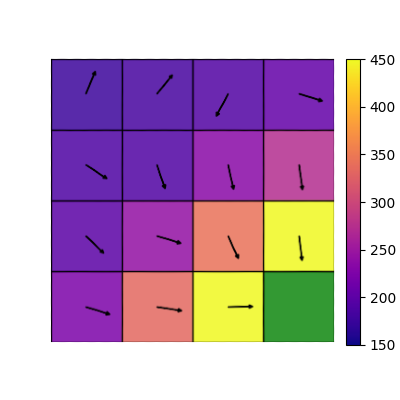
\includegraphics[width=0.6\textwidth]{actorcritic/best}
\end{center}
\caption{Visualization of model policy on a $4 \times 4$ grid after 3000 iterations of 200 ms. Terminal state is colored green. Color of other states shows average weight of connections between the input neuron representing that state and striatum, i.e., expected reward. In each cell, an arrow shows preferred action vector (direction) according to weights between the input neuron and individual output neurons. We see that expected reward from terminal state propagates to more distant states. Directions of state vectors point toward the best action, indicating successful learning, except for the most distant states where the agent, proportionally to expected reward, did not learn an optimal policy.}
\label{results_4x4}
\end{figure}

Similarly to R-STDP, we monitor learning using average reward, but this time reward includes not only external reward but also expected rewards. We expect expected rewards to increase in all states during learning. We verify this with a more direct learning evaluation on the grid, where after each state reset (when we reach goal), we count steps until reaching goal state again. Since different states in which we randomly place the agent are at different distances from the goal, we divide number of steps by Manhattan distance to the goal. This gives ``relative steps''. Average number of relative steps with respect to average weight of all connections between input neurons and striatum neurons over 3000 iterations is shown in graph \ref{progress}, where we see that average number of steps the agent needs to reach the goal decreases proportionally with growth of average expected reward.

\begin{figure}[htbp]
\begin{center}

\includegraphics[width=1.0\textwidth]{actorcritic/progress}
\end{center}
\caption{Average synaptic weight between all input neurons and striatum over 3000 iterations of 200 ms, and average relative number of steps. The figure shows that while average synaptic weight between all input neurons and striatum, representing global expected reward with respect to learned policy, increases, average relative number of steps decreases, reflecting successful learning of a policy approaching optimality.}
\label{progress}
\end{figure}

The implemented system performs so-called ``on-policy'' TD learning, since it updates value of individual states according to value of next state where the next action is selected according to learned policy, unlike so-called ``off-policy'' algorithms where values are updated under the assumption that in the next state we always choose the best action.

\chapter{Conclusion}
The purpose of this thesis was to present and solve some challenges in learning with spiking neural networks. In this thesis, we develop innovative solutions that consider both simulation complexity and meaningfulness from the perspective of neuroscience and real mechanisms in the brain. Additionally, we avoided introducing negative reward, i.e., negative dopamine concentration, since this is not possible in real brains. We thus developed an R-STDP system based solely on competition among synapses, and for problems where we want to avoid certain states, we propose below an extension that does not use negative dopamine concentration. The greatest deviation from a biologically realistic system occurs in searching for system parameters. Parameters were searched only with respect to achieving desired mechanisms, not consistency with values measured in real brains. We allow this also because neuron firing mode, signal transmission through synapses, and neuron configurations as in basal ganglia seem more common across different animal species than neuron and synapse parameters. For example, the center responsible for hearing and vocalization modulation is structurally similar in humans and bats, but in bats these centers clearly operate at much higher frequency. %TODO: verify
Further hyperparameter search could most likely lead to better results than those achieved in this thesis. In systems without recurrent connections and without additional fully connected neuron layers, such as the systems implemented in this thesis, increasing number of neurons in an individual group would not necessarily lead to better results, but this was not tested due to computational cost.

\section{Ideas for Future Work}
\subsection{Aversive Behavior}
\label{aversive}
In most works dealing with reinforcement learning, avoidance of states that we want the agent to avoid is achieved using negative reward. Negative reward in the R-STDP synapse equation flips the update sign, so synapses responsible for entering an undesired state are negatively updated. There is no negative dopamine in the human brain. The idea arises that avoidance of negative states is also a consequence of learning where dopamine level is $n > 0$. Namely, dopamine represents learning, not necessarily reward. Negative reward could be represented by a special input representing a negative stimulus or ``discomfort'' that we want to reduce during learning. Principles of R-STDP and TD learning can again be used, where reduction of discomfort level represents reward. To the current actor-critic system, we would add another critic instance computing temporal difference of discomfort level and acting on dopaminergic neurons shared by both critics. The two critics therefore act competitively. On transition from a state with high negative-stimulus level to one with low level, dopaminergic neurons are excited; in the opposite case they are inhibited. If delivered negative-stimulus level is the same, the negative-reward critic does not influence dopaminergic neurons.

In this case, despite using temporal difference, the system behaves short-sightedly with respect to negative stimulus. Only connections that led us away from discomfort are rewarded, and because negative stimulus is always delivered only from outside the system, rewarded connections appear only in states directly adjacent to the negative state. In contrast, striatum predicts delivered reward level by itself. If we also want to predict discomfort in states near the unpleasant state, we should add another neuron group to the system that associates states with negative stimulus and thus predicts it.

We expect both critics would compete with each other to reward actions that lead closer to reward as well as actions that lead away from negative state.
\begin{figure}[htbp]
\begin{center}
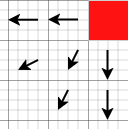
\includegraphics[width=0.4\textwidth]{figures/aversive}
\end{center}
\caption{Expected policy with a negative-state critic (without a rewarded-state critic).}
\label{pic8}
\end{figure}
\subsection{Recurrent Connections}
A major assumption of systems developed in this thesis is the absence of recurrent connections. Therefore states are temporally almost completely independent of each other. If we add more intermediate levels and recurrent connections, states become temporally dependent. In fact, we can no longer define state only by activity of input neurons, since at each moment it also contains information from neurons that fired arbitrarily in the past and carry information about some previous state. In our actor-critic system, at each time $t$ critic would compute temporal difference between two infinitely short states $s_t$ and $s_{t-d}$, where $d$ is delay of direct connection. Nevertheless, we expect the result would not be different, since in the presence of 200 ms stimulation, which so far represented a state, neuronal activity that is a direct consequence of input-neuron stimulation would still dominate in that interval.

In experiments so far, the correct action of a given state was not dependent on actions that brought us to that state, i.e., on state history. In the grid-walking case, we reward terminal state regardless of which state we entered rewarded state from. We expect recurrent connections would be advantageous in tasks where state history matters, i.e., where state reward depends on previous states. If, in grid walking, moving into terminal state from the state above it led to reward but transition from the state on the left did not, terminal state could be treated as two different states depending on transition. A system with recurrent connections, although receiving only information about a concrete cell, would internally represent states dependent also on previous moves.

Recurrent connections also represent an additional challenge. In our actor-critic system, redefinition of current action-selection method would be required, since two output neurons may be connected to each other and always fire together. One solution could be allowing selection of multiple actions at once, where such a situation is ``penalized''.


\iffalse
\chapter{Extra}
\begin{figure}[H]
\begin{center}

\includegraphics[width=1.0\textwidth]{actorcritic/F3 - Learning}
\end{center}
\caption{System behavior during learning on a 3x3 grid. Cells are numbered from left to right, top to bottom. The goal is located at cell 8. Input-to-striatum connections for states 5 and 7 are expectedly the highest, followed by 4, which directly leads to 5 and 7}
\\
\colorbox{Apricot}{%
  \parbox{0.9\linewidth}{%
    \textbf{
      From the above collection of graphs, select excerpts that represent key situations of reward-estimation and learning mechanisms described during training.
    }%
  }%
}

\label{pic8}
\end{figure}

%\cleardoublepage
%\addcontentsline{toc}{chapter}{Literatura}

%\printbibliography[heading=bibintoc,type=article,title={Članki v revijah}]
%https://www.overleaf.com/project/609ce2055f917cb2f776732e
%\printbibliography[heading=bibintoc,type=inproceedings,title={Članki v zbornikih}]
%\printbibliography[heading=bibintoc,type=incollection,title={Poglavja v knjigah}]
\fi
%\printbibliography[heading=bibintoc,title={Viri}]
\bibliographystyle{plainnat}
\bibliography{literatura}

\end{document}
